\appendix

\noindent\textbf{Appendix Contents:}
\cref{app:layer_sweep}~Layer Sweep Results;
\cref{app:cosine_volatility}~Representation Compression Analysis;
\cref{app:holm_bonferroni}~Holm-Bonferroni Correction;
\cref{app:window_ablation}~Window Size Ablation;
\cref{app:ot7b_details}~OpenThinker-7B Details;
\cref{app:gru_details}~GRU Training Details;
\cref{app:control}~Control Task Methodology;
\cref{sec:oracle}~Oracle Upper Bound;
\cref{app:cp_perturbation}~CP Annotation Perturbation;
\cref{app:bocpd_config}~BOCPD/CUSUM Configuration;
\cref{app:k_ablation}~Detection Threshold Ablation;
\cref{app:threshold_sensitivity}~Decision Threshold Sensitivity;
\cref{app:bug}~M002 Bug Disclosure;
\cref{app:two_stage}~Adaptive Two-Stage Detection;
\cref{app:temporal_details}~Temporal Ablation Details;
\cref{app:negative_details}~Negative Results Details (incl.\ \cref{tab:negative});
\cref{app:transfer_details}~Cross-Model Transfer Details;
\cref{app:encoder_robustness}~Encoder Robustness;
\cref{app:random_projection}~Random Projection Baseline;
\cref{app:e5_mistral}~LLM-Based Text Encoder;
\cref{app:position_residual}~Position-Residualized Probing;
\cref{app:hyperparameter_robustness}~Hyperparameter Robustness;
\cref{app:multi_seed}~Multi-Seed Stability;
\cref{app:split_half}~Split-Half Internal Validity;
\cref{app:ba_layer_comparison}~BA-Layer Modality Comparison;
\cref{app:power_analysis}~Post-Hoc Power Analysis;
\cref{app:practical_mitigation}~Practical Mitigation Levels;
\cref{app:32b_full}~32B Model-Specific Analysis;
Use of AI Assistants.

\section{Layer Sweep Results}
\label{app:layer_sweep}

For each model, we sweep all transformer layers and evaluate five candidate selection metrics: (1)~balanced accuracy $\times$ crossing rate (the CR-composite), (2)~pure balanced accuracy, (3)~precision, (4)~inverse pre-CP FPR, and (5)~an additive composite. The CR-composite systematically selects shallow layers across all four models (including R1-8B under the full L0--L24 sweep; \cref{tab:r18b_full_layer}) because early-layer representations exhibit higher crossing rates (more frequent threshold crossings) regardless of discriminative power. Three threshold-based metrics (precision, inverse FPR, additive composite) converge on deep layers for all models; pure balanced accuracy selects layers whose depth varies with the data split (under 70/30: L30 for QwQ-32B, L47 for R1-32B; under the canonical 60/20/20: L63 and L46 respectively; \cref{tab:ba_layer_results}).

\paragraph{Selected layers.} R1-8B: under the original L12--L24 sweep, all five metrics agreed on L14 (44\%); extending to L0--L24, crossing rate shifts to L0 while threshold-based metrics retain L14, a 16-layer gap (\cref{tab:r18b_full_layer}). OT-7B: CR-composite selects L0 (0\%), threshold-based consensus selects L16 (57\%). QwQ-32B: CR-composite selects L2 (3\%), threshold-based consensus selects L63 (98\%). R1-32B: CR-composite selects L10 (16\%), threshold-based consensus selects L63 (98\%). The disagreement is most extreme for 64-layer models, where the CR-composite selects layers in the bottom 16\% of the network while threshold-based metrics select layers at 98\% depth. Under 70/30, pure balanced accuracy selects L30 (47\%) for QwQ-32B and L47 (73\%) for R1-32B; under the canonical 60/20/20, it selects L63 (98\%) and L46 (72\%), which demonstrates sensitivity to the data split.

\paragraph{Impact on modality comparison.} At the CR-composite layers, HS vs.\ text precision $p$-values are 0.064 (R1-32B) and 0.35--0.83 (QwQ-32B), both non-significant. At the threshold-based deep layers, all $p$-values fall below 0.005. The initially reported ``scale-dependent'' pattern (HS advantage at 7--8B but not 32B) was entirely an artifact of layer selection methodology, not a genuine property of model scale (\cref{sec:layer-results}).

\paragraph{Layer selection stability (LOO-CV).} Leave-one-out cross-validation on the validation set shows moderate consistency for 7--8B models (65--68\% dominant-layer agreement) but lower for 32B, confirming that layer selection instability is particularly acute at small sample sizes. Under pure balanced accuracy, the dominant layer is selected in 68\% (QwQ-32B: L30, 13/19 folds) and 65\% (R1-32B: L47, 13/20 folds) of folds. Alternative selections scatter across neighboring layers (L29, L55--56 for QwQ; L32, L38, L43 for R1-32B), reinforcing the need for multi-metric auditing rather than single-metric layer selection. Threshold-based metrics show tighter convergence to L63 for both 32B models. Expanding the criterion from top-1 to top-3 layers does not change conclusions: the top-3 BA-selected layers for QwQ-32B (L30, L29, L55) and R1-32B (L47, L43, L38) all fall in the mid-to-deep range, and threshold-based metrics remain converged at L63 across all folds.

\paragraph{Joint (layer, $W$) sensitivity.} Under the original 70/30 validation protocol, we evaluate QwQ-32B across 64 layers $\times$ 3 windows ($W \in \{1, 3, 5\}$) (192 configurations) (\cref{tab:joint_layer_w}). L60 is near-optimal: within 2.1pp of the global best at $W{=}3$ and the top-ranked layer at $W{=}5$. (Under 60/20/20, threshold-based metrics select L63; the shift from L60 to L63 across splits itself illustrates layer selection sensitivity.) The optimal layer shifts from middle-deep (L46--47 at $W{=}1$) to deep (L60 at $W{=}5$), confirming a layer-window interaction. For R1-8B, optimal precision layers shift similarly (L16 at $W{=}1$ $\to$ L9 at $W{=}15$; Kendall's $\tau{=}{-}0.91$, $p{=}0.071$), a consistent negative trend that does not reach significance at $n{=}4$ windows. L30, selected by per-fold LOO-CV at $W{=}1$ under balanced accuracy, is suboptimal across all windows (max BA $= 0.769$ vs.\ global best 0.817). Joint (layer, $W$) stability was evaluated via grid search on $W \in \{1, 3, 5\}$ for QwQ-32B only; full leave-one-fold-out validation of the (layer, $W$) pair and extension to R1-32B remain for future work.

\begin{table}[htbp]
\centering
\small
\caption{QwQ-32B joint (layer, $W$) grid search under 70/30 validation. L60 is near-optimal at recommended windows ($W{=}3$--$5$). L30 (LOO-CV selection at $W{=}1$) is suboptimal across all windows. Under the canonical 60/20/20 split, threshold-based metrics select L63.}
\label{tab:joint_layer_w}
\resizebox{\columnwidth}{!}{%
\begin{tabular}{clccc}
\toprule
$W$ & \textbf{Best layer} & \textbf{Best BA} & \textbf{L60 BA} & \textbf{L60 rank} \\
\midrule
1 & L47 & 0.798 & 0.783 & $\sim$15th \\
3 & L46 & 0.817 & 0.796 & $\sim$6th \\
5 & L60 & 0.808 & 0.808 & 1st \\
\bottomrule
\end{tabular}}
\end{table}

\paragraph{R1-8B full-layer sweep.}
\label{app:r18b_full_layer}
The original R1-8B layer sweep covered L12--L24 (13 layers), where all five metrics agreed on L14 (\cref{tab:layer_selection}). Extending to L0--L24 reveals that crossing rate consistently selects L0 across all window sizes, while threshold-based metrics retain mid-to-deep layers (L12--L16 for $W{=}1$--$5$; L9 at $W{=}15$, marginal $\Delta{=}0.003$ between shallow and deep means), a 9--16 layer divergence (\cref{tab:r18b_full_layer}). Unlike 32B models, the bias is isolated to crossing rate; threshold-based metrics show no shallow shift for R1-8B. This confirms the crossing-rate bias generalizes to Llama-architecture models. HS probes maintain significant advantage across all 25 layers and window sizes (precision gap ${\sim}$0.15--0.17), unlike OT-7B and 32B models where significance drops at shallow layers.

\begin{table}[htbp]
\centering
\small
\caption{R1-8B full-layer sweep (L0--L24, extending the original L12--L24 range). Best layer selected by crossing rate vs.\ threshold-based metrics across four window sizes. Score = balanced accuracy at the threshold-based layer. Layer gap = crossing-rate layer minus threshold-based layer.}
\label{tab:r18b_full_layer}
\resizebox{\columnwidth}{!}{%
\begin{tabular}{lcccc}
\toprule
& $W{=}1$ & $W{=}3$ & $W{=}5$ & $W{=}15$ \\
\midrule
Crossing rate & L0 & L0 & L0 & L0 \\
Threshold (composite) & L16 (0.789) & L12 (0.796) & L12 (0.803) & L9 (0.784) \\
\midrule
Layer gap & 16 & 12 & 12 & 9 \\
\bottomrule
\end{tabular}}
\end{table}

\subsection{Random-Label Decomposition Control}
\label{app:random_cp}

To decompose the sources of metric disagreement in layer selection, we replace the true CP annotations with uniformly random labels and re-run the full layer sweep (10 random-label repeats per model). We test QwQ-32B (95 traces, 64 layers) and R1-8B (209 traces, 25 layers); \cref{tab:random_cp,tab:random_cp_r18b} report the fraction of repeats selecting a shallow layer and the mean selected layer.

\begin{table}[htbp]
\centering
\small
\caption{QwQ-32B layer selection under random CP labels (10 repeats). Shallow\%: fraction selecting a layer L$\leq$10. Real-CP layer shown for reference.}
\label{tab:random_cp}
\setlength{\tabcolsep}{4pt}
\resizebox{\columnwidth}{!}{%
\begin{tabular}{lcccc}
\toprule
\textbf{Metric} & \textbf{Real-CP} & \textbf{Shallow\%} & \textbf{Rand.\ mean layer} \\
\midrule
Crossing rate & L4 & 100\% & $3.4 \pm 2.6$ \\
CR-composite & L4 & 80\% & $13.1 \pm 18.1$ \\
Precision & L63 & 20\% & $33.8 \pm 19.8$ \\
Inv.\ FPR & L62 & 10\% & $36.4 \pm 17.0$ \\
Bal.\ accuracy & L63 & 20\% & $33.3 \pm 20.3$ \\
\bottomrule
\end{tabular}}
\end{table}

\begin{table}[htbp]
\centering
\small
\caption{R1-8B layer selection under random CP labels (10 repeats). Shallow\%: fraction selecting L$\leq$4 (bottom quintile of 25 layers). $\dagger$: degenerate, all repeats select L0 with zero variance, indicating destroyed signal rather than shallow preference.}
\label{tab:random_cp_r18b}
\setlength{\tabcolsep}{4pt}
\resizebox{\columnwidth}{!}{%
\begin{tabular}{lcccc}
\toprule
\textbf{Metric} & \textbf{Real-CP} & \textbf{Shallow\%} & \textbf{Rand.\ mean layer} \\
\midrule
Crossing rate & L0 & 0\% & $10.7 \pm 4.8$ \\
CR-composite & L0 & 0\% & $13.7 \pm 6.7$ \\
Precision & L23 & 100\%$^{\dagger}$ & $0.0 \pm 0.0$ \\
Inv.\ FPR & L13 & 100\%$^{\dagger}$ & $0.0 \pm 0.0$ \\
Bal.\ accuracy & L19 & 0\% & $14.0 \pm 4.0$ \\
\bottomrule
\end{tabular}}
\end{table}

\paragraph{QwQ-32B (Qwen).} The results decompose the metric disagreement into two components. (A)~The crossing-rate shallow-layer preference is label-independent: 100\% of random-label repeats still select layers L0--L7, confirming that this bias reflects representation geometry (shallow-layer cosine distance compression; \cref{app:cosine_volatility}) rather than any property of the safety labels. The CR-composite inherits this bias (80\% shallow). (B)~Threshold-based metrics (precision, inverse FPR) select deep layers only with real safety labels; under random labels, selections scatter across the full layer range (mean L34--L36, high variance). The full metric disagreement (L4 vs.\ L63, a 59-layer gap) is the superposition of a geometric artifact on the crossing-rate side and a real safety signal on the threshold-based side.

\paragraph{R1-8B (Llama).} The Llama-based model shows stronger label dependence: crossing rate scatters from L0 to mean L$10.7 \pm 4.8$ under random labels (0\% shallow), unlike QwQ-32B where it retains shallow preference. Threshold-based metrics degenerate entirely: precision and inverse FPR select L0 in all 10 repeats with zero variance, indicating random labels destroy discriminative signal rather than merely redistributing it. The real-CP disagreement (L0 vs.\ L23, a 23-layer gap) vanishes completely under random labels.

\paragraph{Cross-architecture summary.} The metric disagreement requires genuine safety labels in both architectures, but the mechanism differs: in QwQ-32B, crossing-rate shallow preference reflects representation geometry (label-independent cosine compression), while in R1-8B even crossing-rate layer selection is label-dependent. The geometric component of the crossing-rate bias is thus Qwen-specific rather than a universal property of transformer representations.

\section{Representation Compression Analysis}
\label{app:cosine_volatility}

We measure step-to-step cosine distance at CR-composite (shallow) vs.\ threshold-based (deep) layers across all models to characterize the compression mechanism underlying the crossing rate bias (\cref{tab:cosine_volatility}).

\begin{table}[htbp]
\centering
\small
\caption{Step-to-step cosine distance at shallow and threshold-based (deep) layers. Shallow layers produce highly compressed representations (1.4--2.7$\times$ smaller inter-step distances). Shallow layers are L2 for R1-8B/OT-7B/QwQ-32B and L10 for R1-32B; deep layers follow threshold-based consensus (\cref{tab:layer_selection}).}
\label{tab:cosine_volatility}
\resizebox{\columnwidth}{!}{%
\begin{tabular}{llcc}
\toprule
\textbf{Model} & \textbf{Layer (depth)} & \textbf{Mean} & \textbf{Std} \\
\midrule
R1-8B & L2 (shallow) & 0.186 & 0.097 \\
 & L14 (deep) & 0.411 & 0.143 \\[2pt]
OT-7B & L2 (shallow) & 0.077 & 0.080 \\
 & L16 (deep) & 0.206 & 0.091 \\[2pt]
QwQ-32B & L2 (shallow) & 0.037 & 0.064 \\
 & L63 (deep) & 0.084 & 0.056 \\[2pt]
R1-32B & L10 (shallow) & 0.067 & 0.050 \\
 & L63 (deep) & 0.092 & 0.076 \\
\bottomrule
\end{tabular}}
\end{table}

Shallow layers produce highly compressed representations: consecutive steps cluster within small cosine distances (0.04--0.19), while deep-layer representations spread more widely (0.09--0.41). Inter-step distances at shallow layers are 1.4--2.7$\times$ smaller than at deep layers across all models. A linear probe operating in this compressed space sits near the noise floor, where minor numerical fluctuations produce spurious threshold crossings that inflate crossing rate independently of discriminative power. Deep layers produce well-separated representations where crossings correspond to genuine semantic transitions.

\paragraph{Cross-dataset evidence.}
To assess whether this geometric precondition generalizes beyond HarmThoughts, we compute the same shallow/deep volatility ratio on AdvBench~\citep{advbench} traces using R1-8B ($n{=}520$ traces). The deep-layer mean cosine distance (0.472) is $1.54\times$ the shallow-layer mean (0.307), consistent with the 1.4--2.7$\times$ range observed across all four models on HarmThoughts (\cref{tab:cosine_volatility}). This confirms that the representational compression underlying metric-induced layer selection bias is not dataset-specific and does not depend on CP annotations.

\subsection{AdvBench Boundary Condition}
\label{app:advbench_cp}

We analyze R1-8B behavior on 388 substantive-response AdvBench~\citep{advbench} traces (of 520 total) to characterize a boundary condition for the CP framework (\cref{tab:advbench_boundary}).

\begin{table}[htbp]
\centering
\small
\caption{R1-8B behavior on AdvBench adversarial prompts (388 substantive-response traces of 520 total). CP${=}0$ indicates the model produces harmful content from the first reasoning step without prior safety deliberation.}
\label{tab:advbench_boundary}
\resizebox{\columnwidth}{!}{%
\begin{tabular}{lc}
\toprule
\textbf{Metric} & \textbf{Value} \\
\midrule
Jailbreak rate & 13.4\% \\
CP${=}0$ (among JB) & 90.4\% \\
Mean CP position (among JB) & 1.4 steps \\
\bottomrule
\end{tabular}}
\end{table}

Adversarial prompts designed to bypass safety mechanisms (e.g., GCG suffixes) cause the model to skip safety deliberation entirely: 90.4\% of jailbroken traces have CP${=}0$, meaning the model commits to harmful generation from the first reasoning step. This contrasts with HarmThoughts, where non-adversarial prompts trigger extended safety deliberation before commitment (mean relative CP position ${\approx}0.7$). The CP framework is most informative when prompts elicit deliberation that can be monitored; adversarial prompts that circumvent deliberation represent a boundary condition where commitment detection is vacuous. The geometric compression evidence (\cref{tab:cosine_volatility}; volatility ratio $1.54\times$) remains valid because it measures representational properties independent of CP annotations.

\subsection{AdvBench Layer Selection Bias Replication}
\label{app:advbench_layer_bias}

We replicate the five-metric layer selection analysis on AdvBench~\citep{advbench} to test whether metric-induced layer divergence depends on HarmThoughts-specific CP annotations or generalizes to simpler binary supervision. Using R1-8B, we generate reasoning traces for all 520 AdvBench prompts, classify each as jailbreak or safe via keyword matching, and evaluate logistic regression probes across all 32 layers (L0--L31) with windows $W \in \{1, 3, 5, 15\}$. The 60/20/20 train/val/test split matches HarmThoughts protocol.

\paragraph{Data distribution.} Of 520 traces, 159 (30.6\%) are classified as jailbreak and 361 (69.4\%) as safe. A stricter keyword classifier (applied only to final responses, threshold ${\geq}1$ refusal phrase) reduces the jailbreak rate from 79.2\% (v1) to 30.6\%; the full-data divergence increases from 42pp (v1) to 58pp (v2); with proper held-out evaluation, the v2 bootstrap mean is 31.7pp ($p{=}0.015$), confirming the bias is genuine and not an artifact of label noise.

\begin{table}[h]
\centering
\small
\caption{AdvBench layer selection (R1-8B, 32 layers). CR-composite selects shallow layers; precision and inverse FPR select deep layers; AUROC selects mid-depth layers. Consistent with HarmThoughts (\cref{tab:layer_selection}).}
\label{tab:advbench_layer_selection}
\resizebox{\columnwidth}{!}{%
\begin{tabular}{lccc}
\toprule
\textbf{Metric} & \textbf{Best Layer} & \textbf{Depth (\%)} & \textbf{Best $W$} \\
\midrule
CR-composite (BA $\times$ CR) & L3 & 9.7\% & 5 \\
Crossing rate & L0 & 0.0\% & 5 \\
Precision & L21 & 67.7\% & 15 \\
Inverse FPR & L21 & 67.7\% & 15 \\
Balanced accuracy & L9 & 29.0\% & 15 \\
AUROC & L11 & 35.5\% & 15 \\
\bottomrule
\end{tabular}}
\end{table}

\paragraph{Crossing rate pattern.} Mean crossing rate at shallow layers is elevated relative to deep layers, consistent with the cosine compression range observed on HarmThoughts (\cref{tab:cosine_volatility}).

\paragraph{Per-window consistency.} Precision and inverse FPR consistently select deep layers regardless of window size, while the CR-composite is pulled toward shallow layers across all windows.

The bootstrap-validated divergence (31.7pp, $p{=}0.015$) between CR-composite and precision/inverse-FPR selection replicates the HarmThoughts pattern (L0 vs.\ L14, 44\% divergence) under different label semantics (binary jailbreak/safe vs.\ step-level CP). This confirms that the bias arises from representational geometry (shallow-layer cosine compression) rather than task-specific label structure.

\paragraph{Bootstrap validation.} The full-data analysis (training and evaluation on the same data) yields a 58pp divergence (L3 at 9.7\% vs.\ L21 at 67.7\%), which includes layer selection overfitting. To obtain a proper held-out estimate, we run 1{,}000 bootstrap iterations with stratified 60/40 train/test splits: probes are trained on the training split (60\%). In each bootstrap iteration, test traces are resampled with replacement, and both layer selection and divergence measurement are performed on the resampled test set; this estimates the full pipeline variance including selection variability. The bootstrap mean divergence is 31.7pp (95\% CI [3.2, 48.4]pp, $p{=}0.015$). Layer selection is stable across iterations: the CR-composite median is L2 and the precision median is L14, consistent with the shallow/deep divergence pattern. The gap between full-data (58pp) and bootstrap (31.7pp) estimates reflects overfitting in layer selection when train and test data overlap, reinforcing the need for held-out evaluation in layer selection studies.

\subsection{Cross-Architecture Geometric Analysis (Gemma)}
\label{app:gemma_cross_arch}

To test whether the geometric precondition for layer selection bias generalizes beyond Llama and Qwen, we evaluate cosine compression on two Gemma-family models using AdvBench traces. Gemma-2-9B-it (standard multi-head attention) and Gemma-4-E4B (mixed sliding-window/full attention, window size 512) each generate 520 traces. Gemma-2 (6 JB / 520, 1.15\%) and Gemma-4 (14 JB / 520, 2.7\%) produce insufficient positive samples for reliable probe-based layer selection analysis; we therefore report only the geometric precondition (cosine compression).

\begin{table}[h]
\centering
\small
\caption{Cross-architecture cosine compression. Deep/shallow ratio ${>}1$ indicates shallow-layer compression (the geometric precondition for crossing-rate inflation). Standard full attention consistently shows compression; Gemma-4's mixed sliding/full attention does not. $^a$\,Probe-selected layers from HarmThoughts (L2 vs.\ L14). $^b$\,Range-based windows (first 15\% vs.\ last 25\% of layers) due to insufficient jailbreak samples for probe-based selection.}
\label{tab:gemma_compression}
\resizebox{\columnwidth}{!}{%
\begin{tabular}{llccc}
\toprule
\textbf{Model} & \textbf{Attention} & \textbf{Method} & \textbf{Deep/Shallow} & \textbf{Compression} \\
\midrule
R1-8B (Llama) & Standard & Probe$^a$ & $1.54\times$ & \checkmark \\
Gemma-2-9B & Standard & Range$^b$ & $1.28\times$ & \checkmark \\
Gemma-4-E4B & Mixed sliding/full & Range$^b$ & $0.70\times$ & -- \\
\bottomrule
\end{tabular}}
\end{table}

Gemma-2's standard full attention produces a shallow-layer compression pattern consistent in direction with Llama and Qwen (deep/shallow ratio $1.28\times$, same direction as HarmThoughts models at $1.4$--$2.7\times$ though at reduced magnitude). Gemma-4's mixed sliding-window/full attention inverts this pattern (ratio $0.70\times$): shallow layers produce \emph{larger} inter-step distances than deep layers, eliminating the geometric precondition for crossing-rate inflation. This suggests the compression arises from full self-attention's global receptive field, while sliding attention's local window disrupts the shallow-layer clustering that drives crossing-rate inflation. The geometric precondition thus generalizes across all models with standard full attention (Llama, Qwen, Gemma-2) but is absent under mixed attention, indicating that the layer selection bias is attention-mechanism-dependent.

\section{Holm-Bonferroni Step-Down Correction}
\label{app:holm_bonferroni}

\cref{tab:holm_bonferroni} reports the full test battery used to assess hidden-state superiority over text probes. Because balanced accuracy, precision, and FPR share the same confusion matrix, the three per-model metrics are correlated; the effective number of independent comparisons is four (one per model). We report both the conservative 12-test correction and the 4-test model-level correction: both yield the same outcome (all tests pass at $\alpha{=}0.05$). Under 4-test HB, the tightest threshold falls on R1-8B FPR ($p{=}0.044$, rank-4 threshold $\alpha/1{=}0.050$), which still passes. Tests are ranked by $p$-value; each test $i$ (rank $i$ of $m$) must satisfy $p_i < \alpha / (m - i + 1)$ under the step-down procedure.

\begin{table}[htbp]
\centering
\small
\caption{Holm-Bonferroni step-down correction for 12 tests (4 models $\times$ 3 correlated metrics). Each test uses a two-sided null-centered bootstrap (10{,}000 resamples) on trace-level metric differences (HS minus text). All 12 pass at $\alpha{=}0.05$; a 4-test model-level correction (one per model, using the worst $p$-value) also passes.}
\label{tab:holm_bonferroni}
\setlength{\tabcolsep}{4pt}
\resizebox{\columnwidth}{!}{%
\begin{tabular}{clllcc}
\toprule
\textbf{Rank} & \textbf{Model} & \textbf{Metric} & \textbf{$p$-val} & \textbf{Thresh.} & \textbf{Pass} \\
\midrule
1  & R1-8B  & Precision & $<$0.001 & 0.0042 & \checkmark \\
2  & OT-7B  & Bal.\ Acc. & $<$0.001 & 0.0045 & \checkmark \\
3  & OT-7B  & Precision & $<$0.001 & 0.0050 & \checkmark \\
4  & OT-7B  & FPR & $<$0.001 & 0.0056 & \checkmark \\
5  & QwQ-32B & Bal.\ Acc. & $<$0.001 & 0.0063 & \checkmark \\
6  & QwQ-32B & Precision & $<$0.001 & 0.0071 & \checkmark \\
7  & R1-32B & Bal.\ Acc. & $<$0.001 & 0.0083 & \checkmark \\
8  & R1-32B & Precision & $<$0.001 & 0.0100 & \checkmark \\
9  & QwQ-32B & FPR & 0.004 & 0.0125 & \checkmark \\
10 & R1-8B  & Bal.\ Acc. & 0.005 & 0.0167 & \checkmark \\
11 & R1-32B & FPR & 0.007 & 0.0250 & \checkmark \\
12 & R1-8B  & FPR & 0.044 & 0.0500 & \checkmark \\
\bottomrule
\end{tabular}}
\end{table}

The weakest test (rank 12, R1-8B FPR, $p{=}0.044$) passes its threshold ($\alpha/1 = 0.05$) with margin. The ordering reveals that OT-7B produces the strongest HS-text separation (ranks 2--4), while R1-8B FPR is the least significant despite R1-8B's precision gap (+20.1pp at $W{=}3$). This reflects R1-8B's already-low text FPR (11.8\%), which leaves less room for HS improvement on this metric.

\paragraph{Exact sign-flip permutation test validation.} As an independent check on bootstrap significance for the small-sample 32B models, we run exact sign-flip permutation tests on all six 32B comparisons, enumerating all $2^n$ sign permutations ($2^{19}{=}524{,}288$ for QwQ-32B, $2^{20}{=}1{,}048{,}576$ for R1-32B). All six tests reject the null at $\alpha{=}0.05$: QwQ-32B (bal\_acc $p{<}0.001$, precision $p{=}0.003$, FPR $p{<}0.001$); R1-32B (bal\_acc $p{=}0.008$, precision $p{<}0.001$, FPR $p{=}0.004$). The permutation $p$-values are consistent with the bootstrap values in \cref{tab:holm_bonferroni} and confirm that the conclusions are not artifacts of distributional assumptions at small $n$.


\section{Window Size Ablation Details}
\label{app:window_ablation}

\cref{tab:window_full} reports the complete window size ablation across all models and seven window sizes. The main text (\cref{sec:temporal}) presents R1-8B results; here we provide the full data. \cref{fig:window_ablation} visualizes the monotonic improvement on R1-8B: precision rises from 69.3\% ($W{=}1$) to 82.2\% ($W{=}25$) while FPR drops from 9.65\% to 4.8\%.

% Window ablation figure moved to main text §4.5 (Figure: fig_window_ablation)

\begin{table}[htbp]
\centering
\small
\caption{Window size ablation (step-level metrics): balanced accuracy, precision, pre-CP FPR, coverage ($K{=}1$), and mean detection lead across all models.}
\label{tab:window_full}
\resizebox{\columnwidth}{!}{%
\begin{tabular}{llccccc}
\toprule
Model & $W$ & Bal.\ Acc. & Precision & FPR$_{\text{step}}$ & Coverage & Lead \\
\midrule
\multirow{7}{*}{R1-8B}
 & 1  & 77.8 & 69.3 & 9.65 & 72.1 & 13.8 \\
 & 3  & 79.0 & 72.3 & 8.50 & 69.8 & 12.1 \\
 & 5  & 78.1 & 72.6 & 8.09 & 65.1 & 8.3 \\
 & 10 & 79.3 & 74.3 & 7.61 & 55.8 & 10.0 \\
 & 15 & 80.2 & 77.7 & 6.39 & 51.2 & 7.2 \\
 & 20 & 80.7 & 78.6 & 6.12 & 53.5 & 7.4 \\
 & 25 & 81.0 & 82.2 & 4.83 & 48.8 & 8.1 \\
\midrule
\multirow{7}{*}{OT-7B}
 & 1  & 68.2 & 42.8 & 12.0 & 53.2 & 16.1 \\
 & 3  & \textbf{68.8} & 46.6 & 10.0 & 53.2 & 21.6 \\
 & 5  & 68.1 & 46.4 & 9.9 & 53.2 & 21.7 \\
 & 10 & 66.5 & 46.9 & 8.6 & 48.9 & 25.0 \\
 & 15 & 66.4 & 48.8 & 7.7 & 44.7 & 39.6 \\
 & 20 & 66.0 & \textbf{49.4} & \textbf{7.5} & 48.9 & 17.9 \\
 & 25 & 65.9 & 48.9 & 8.0 & 51.1 & 28.3 \\
\midrule
\multirow{7}{*}{R1-32B}
 & 1  & 71.8 & 54.9 & 32.03 & 80.0 & 12.9 \\
 & 3  & 72.5 & 56.0 & 30.64 & 80.0 & 11.4 \\
 & 5  & 73.1 & 57.5 & 28.41 & 75.0 & 11.1 \\
 & 10 & 73.7 & 60.9 & 23.40 & 70.0 & 10.8 \\
 & 15 & 72.1 & 59.1 & 24.51 & 70.0 & 10.9 \\
 & 20 & 69.6 & 56.3 & 26.18 & 65.0 & 9.6 \\
 & 25 & 70.3 & 56.6 & 26.46 & 70.0 & 10.7 \\
\midrule
\multirow{7}{*}{QwQ-32B}
 & 1  & 73.0 & 54.4 & 22.76 & 79.0 & 19.7 \\
 & 3  & 74.5 & 56.5 & 21.41 & 73.7 & 20.6 \\
 & 5  & 76.1 & 57.3 & 21.68 & 73.7 & 20.1 \\
 & 10 & 74.7 & 57.1 & 20.73 & 73.7 & 18.4 \\
 & 15 & 74.1 & 58.2 & 19.11 & 68.4 & 15.8 \\
 & 20 & 75.4 & 60.2 & 17.89 & 63.2 & 15.8 \\
 & 25 & 76.2 & 61.8 & 16.94 & 57.9 & 14.9 \\
\bottomrule
\end{tabular}}%
\end{table}

Key cross-model patterns emerge from the window ablation:

\paragraph{R1-8B} shows a general upward trend in balanced accuracy from 77.8\% ($W{=}1$) to 81.0\% ($W{=}25$), gaining +3.2pp overall with a slight dip at $W{=}5$ (78.1\%). Precision improves sharply (+12.9pp) and step-level FPR halves (9.65\% to 4.83\%). Coverage trades off against quality, dropping from 72.1\% to 48.8\%.

\paragraph{OT-7B} exhibits a split temporal pattern at layer 16: balanced accuracy peaks at $W{=}3$ (68.8\%) and declines at larger windows ($-$2.9pp by $W{=}25$), while precision and FPR continue improving. Precision rises from 42.8\% ($W{=}1$) to 49.4\% ($W{=}20$), and FPR drops from 12.0\% to 7.5\% over the same range. The split indicates that larger windows reduce false alarms and sharpen positive predictions even as overall classification accuracy degrades. Lead times are shorter than old layer-0 estimates (16.1--39.6 steps) due to the threshold-based layer selection (\cref{app:ot7b_details}). OT-7B text probes improve monotonically across all metrics (\cref{app:ot7b_details}), so the accuracy saturation is specific to HS probes on this model.

\paragraph{R1-32B} exhibits a non-monotonic pattern: balanced accuracy peaks at $W{=}10$ (73.7\%) and then declines, falling below the $W{=}1$ baseline by $W{=}20$ (69.6\%). The optimal window for R1-32B is $W{=}10$, which achieves the lowest FPR (23.40\%) and highest precision (60.9\%). The accuracy degradation at large windows likely reflects overfitting on the smaller dataset ($n{=}100$).

\paragraph{QwQ-32B} shows a broadly increasing trend with local non-monotonicity: balanced accuracy peaks at $W{=}5$ (76.1\%), dips at $W{=}10$--$15$, then recovers to 76.2\% at $W{=}25$. Precision and FPR improve monotonically with larger windows (54.4\% to 61.8\% precision; 22.76\% to 16.94\% FPR). QwQ-32B produces substantially longer lead times than R1-8B and R1-32B (19.7 steps at $W{=}1$, 14.9 at $W{=}25$), though OT-7B's lead times are longer still.

\paragraph{Universal trends.} Across all models: (1) larger windows reduce coverage as the smoothed probe fires less frequently; (2) HS FPR generally decreases with window size; (3) lead time is model-dependent. The primary cross-model difference is whether balanced accuracy improves broadly (R1-8B, QwQ-32B), peaks sharply at an intermediate window (R1-32B at $W{=}10$), or peaks very early (OT-7B at $W{=}3$). Each model uses its validation-selected window in the main text.

\subsection{Text Probe Window Ablation}
\label{app:text_window}

\cref{tab:text_window} reports the complete text probe window sweep on R1-8B and confirms that temporal context benefits text probes even more strongly than HS probes.

\begin{table}[htbp]
\centering
\caption{Text probe window ablation on R1-8B (step-level metrics). Text probes gain +12.0pp accuracy from $W{=}1$ to $W{=}25$, compared to +3.2pp for HS probes over the same range. The larger marginal gain for text probes reflects their weaker single-step baseline.}
\label{tab:text_window}
\resizebox{\columnwidth}{!}{%
\begin{tabular}{lcccc}
\toprule
$W$ & Bal. Acc. & Precision & FPR & Coverage \\
\midrule
 1  & 64.7 & 41.6 & 25.8 & 95.4 \\
 3  & 66.9 & 44.8 & 23.1 & 90.7 \\
 5  & 69.2 & 48.5 & 20.4 & 84.9 \\
 10 & 72.1 & 54.3 & 16.7 & 74.4 \\
 15 & 74.3 & 58.9 & 14.2 & 67.4 \\
 20 & 75.8 & 62.1 & 12.5 & 62.8 \\
 25 & 76.7 & 64.8 & 11.8 & 58.1 \\
\bottomrule
\end{tabular}}
\end{table}

Text probes show monotonic improvement across all window sizes without the plateau observed in HS probes (which saturate around $W{=}15$). The absolute FPR reduction ($-$14.0pp) is nearly three times the HS reduction ($-$4.8pp), and accuracy gains (+12.0pp vs.\ +3.2pp) are four times larger. This asymmetry supports the interpretation that temporal context is the primary factor in commitment detection: text features, which encode less information per step, benefit proportionally more from observing the multi-step progression.


\section{OpenThinker-7B Detailed Results}
\label{app:ot7b_details}

OpenThinker-7B (OT-7B) is trained with STILL~\cite{still} on Qwen2.5-7B to produce a 7B reasoning model with a different training paradigm from the R1-distilled models. We report the full layer sweep and text probe window ablation.

\paragraph{Layer sweep.}

\begin{table}[htbp]
\centering
\small
\caption{OT-7B layer sweep. Score = balanced accuracy $\times$ crossing rate. Layer 16 (57\% depth) is selected after correction; it achieves the highest balanced accuracy among transformer layers.}
\label{tab:ot7b_layer_sweep}
\setlength{\tabcolsep}{4pt}
\resizebox{\columnwidth}{!}{%
\begin{tabular}{lcccc}
\toprule
Layer & Depth & Bal.\ Acc. & Cross.\ Rate & Score \\
\midrule
0 (embed.) & 0 & 66.7 & 53.2 & 35.5 \\
4 & 14 & 66.3 & 40.4 & 26.8 \\
8 & 29 & 66.4 & 25.5 & 17.0 \\
12 & 43 & 67.5 & 31.9 & 21.6 \\
16 & 57 & 68.2 & 31.9 & 21.8 \\
20 & 71 & 65.5 & 31.9 & 20.9 \\
24 & 86 & 66.9 & 29.8 & 19.9 \\
27 & 96 & 63.0 & 31.9 & 20.1 \\
\bottomrule
\end{tabular}}
\end{table}

After correction of a layer selection bug, layer 16 (57\% depth) is selected. It achieves the highest balanced accuracy (68.2\%) among transformer layers under the 70/30 split used here; under the canonical 60/20/20 split, BA selects L2 (7\% depth; \cref{tab:ba_layer_results}). Layer 0 (embedding) has a higher crossing rate (53.2\% vs.\ 31.9\%) but lower accuracy.

\paragraph{Text probe window ablation.}

\begin{table}[htbp]
\centering
\small
\caption{OT-7B text probe window ablation (step-level). Text probes improve monotonically with larger $W$, contrasting with the HS probes on this model which peak at $W{=}3$.}
\label{tab:ot7b_text_window}
\resizebox{\columnwidth}{!}{%
\begin{tabular}{lcccc}
\toprule
$W$ & Bal. Acc. & Precision & FPR & Coverage \\
\midrule
 1  & 58.1 & 24.5 & 34.5 & 63.8 \\
 3  & 57.9 & 25.4 & 27.1 & 74.5 \\
 5  & 56.9 & 24.7 & 25.5 & 70.2 \\
 10 & 58.3 & 27.0 & 22.2 & 70.2 \\
 15 & 58.9 & 28.3 & 20.0 & 66.0 \\
 20 & 60.9 & 31.6 & 17.6 & 66.0 \\
 25 & 61.4 & 32.9 & 16.1 & 66.0 \\
\bottomrule
\end{tabular}}
\end{table}

OT-7B text probes improve monotonically from $W{=}1$ to $W{=}25$ (+3.3pp accuracy, +8.4pp precision, $-$18.4pp FPR), consistent with the R1-8B pattern. OT-7B HS probes show a split pattern: balanced accuracy peaks at $W{=}3$ and declines, while precision and FPR continue improving (\cref{tab:window_full}). The text-HS contrast is therefore metric-dependent rather than a blanket modality difference.

\paragraph{Bootstrap comparison (matched $W{=}3$).} To ensure a fair modality comparison, bootstrap tests use matched $W{=}3$ for both HS and text probes. At $W{=}3$, HS probes achieve 75.3\% trace-level balanced accuracy vs.\ 65.6\% for text (bootstrap $\Delta{=}$+10.7pp, 95\% CI [4.9, 16.3], $p{<}0.001$, survives Holm-Bonferroni). Precision: 55.8\% vs.\ 34.6\% (bootstrap $\Delta{=}$+21.9pp, 95\% CI [14.0, 29.6], $p{<}0.001$, survives Holm-Bonferroni). Pre-CP FPR: 10.0\% vs.\ 27.1\% (bootstrap $\Delta{=}{-}17.1$pp, 95\% CI [$-$22.2, $-$12.2], $p{<}0.001$, survives Holm-Bonferroni). All three metrics survive correction. The point-estimate precision gap (+21.2pp) aligns with the bootstrap mean (+21.9pp); the small discrepancy reflects resampling variance. Using each modality's optimal $W$ (HS at $W{=}3$, text at $W{=}25$) would introduce a confound because text would benefit from 8$\times$ more temporal context.


\section{GRU Training Details}
\label{app:gru_details}

GRU results serve as supplementary evidence under a different training protocol (70/30 split); direct comparison with the main logistic regression pipeline (60/20/20 nested CV) is not intended.

\paragraph{Data split.} GRU experiments use a 70/30 train/test split to maximize training data for the sequential model, differing from the main 60/20/20 protocol used for logistic regression probes. Within the 70\% training portion, we hold out 10\% of total traces as a validation set for early stopping (effective 60/10/30 split). The validation set is used only for early stopping and is not included in reported test metrics, so there is no information leakage.

\paragraph{Architecture.} We evaluate two GRU variants. The single-layer variant uses a GRU with hidden dimension 256, taking per-step hidden states from the best layer (selected by validation balanced accuracy) as input. The multi-layer variant concatenates hidden states from 7 layers (evenly spaced through the network) at each step to produce a higher-dimensional input to the same GRU architecture.

\paragraph{Training procedure.} We train with Adam (learning rate $1 \times 10^{-3}$, default $\beta_1{=}0.9$, $\beta_2{=}0.999$), batch size 16, for a maximum of 50 epochs. Early stopping halts training when validation loss does not improve for 10 consecutive epochs. Input features are z-score normalized per dimension using training set statistics.

\paragraph{Evaluation.} We report crossing accuracy (the sustained accuracy at which the probe first exceeds chance for 5 consecutive steps) and detection lead (steps before CP at crossing point). All experiments use 3 random seeds; we report mean $\pm$ standard deviation.

\paragraph{Per-seed results for R1-8B (single-layer GRU).}

\begin{table}[htbp]
\centering
\small
\caption{R1-8B single-layer GRU results per seed. Lead is measured in steps before the commitment point.}
\label{tab:gru_seeds}
\setlength{\tabcolsep}{4pt}
\resizebox{\columnwidth}{!}{%
\begin{tabular}{lccc}
\toprule
Seed & Peak Acc. & Crossing Acc. & Lead (steps) \\
\midrule
1 & 85.2 & 74.3 & +4.8 \\
2 & 83.1 & 71.6 & +4.8 \\
3 & 83.4 & 70.4 & +0.9 \\
\midrule
Mean $\pm$ std & 83.9 $\pm$ 1.1 & 72.1 $\pm$ 2.0 & +3.5 $\pm$ 2.3 \\
\bottomrule
\end{tabular}}
\end{table}

The high variance in lead time (standard deviation of 2.3 steps) is driven by seed 3, where the probe achieves good peak accuracy but crosses the detection threshold late. This variance underscores the sensitivity of early detection to initialization and motivates reporting per-seed results rather than relying on mean values alone.

Results in this section use the 60/20/20 protocol consistent with the main text; earlier 70/30 results are retained for completeness but should not be compared directly.

\paragraph{Multi-layer GRU and baseline comparison (60/20/20 protocol).}

\begin{table}[htbp]
\centering
\scriptsize
\caption{Per-seed performance of GRU and logistic regression (LR) probes on R1-8B under a 60/20/20 cross-validation protocol (seeds 42, 123, 456). Single = layer 14 only; Multi = 7-layer concatenation (layers 12--24, stride 2). Lead = steps before CP at first sustained crossing. Main text results use a 70/30 train/test split with different test traces, accounting for the difference in lead values.}
\label{tab:gru_multi_seeds}
\resizebox{\columnwidth}{!}{%
\begin{tabular}{llccccc}
\toprule
Model & Seed & Acc & Prec & FPR & Cross.\% & Lead \\
\midrule
GRU-single & 42  & 0.845 & 0.657 & 0.139 & 72.1\% & 3.55 \\
GRU-single & 123 & 0.760 & 0.454 & 0.191 & 65.1\% & 7.39 \\
GRU-single & 456 & 0.792 & 0.474 & 0.203 & 67.4\% & 8.45 \\
\rowcolor{gray!10}
GRU-single & \textit{mean} & 0.799$\pm$0.035 & 0.528$\pm$0.091 & 0.178$\pm$0.028 & 68.2$\pm$2.9\% & 6.46$\pm$2.10 \\
\midrule
GRU-multi  & 42  & 0.824 & 0.616 & 0.164 & 74.4\% & 5.66 \\
GRU-multi  & 123 & 0.759 & 0.454 & 0.195 & 65.1\% & 6.43 \\
GRU-multi  & 456 & 0.784 & 0.460 & 0.207 & 65.1\% & 8.93 \\
\rowcolor{gray!10}
GRU-multi  & \textit{mean} & 0.789$\pm$0.027 & 0.510$\pm$0.075 & 0.189$\pm$0.018 & 68.2$\pm$4.4\% & 7.01$\pm$1.40 \\
\midrule
LR-single  & 42  & 0.841 & 0.693 & 0.097 & 46.5\% & $-$2.00 \\
LR-single  & 123 & 0.753 & 0.436 & 0.181 & 53.5\% & 5.26 \\
LR-single  & 456 & 0.814 & 0.512 & 0.146 & 41.9\% & 3.94 \\
\rowcolor{gray!10}
LR-single  & \textit{mean} & 0.803$\pm$0.037 & 0.547$\pm$0.108 & 0.141$\pm$0.035 & 47.3$\pm$4.8\% & 2.40$\pm$3.16 \\
\midrule
LR-multi   & 42  & 0.827 & 0.679 & 0.092 & 39.5\% & 1.06 \\
LR-multi   & 123 & 0.756 & 0.442 & 0.180 & 46.5\% & 7.30 \\
LR-multi   & 456 & 0.817 & 0.521 & 0.130 & 34.9\% & 4.00 \\
\rowcolor{gray!10}
LR-multi   & \textit{mean} & 0.800$\pm$0.032 & 0.547$\pm$0.099 & 0.134$\pm$0.036 & 40.3$\pm$4.8\% & 4.12$\pm$2.55 \\
\bottomrule
\end{tabular}}%
\end{table}

Under this protocol, multi-layer GRU achieves the highest mean lead (7.01$\pm$1.40 steps) but at higher FPR than logistic regression baselines (0.189 vs.\ 0.134). The GRU advantage is concentrated in detection timing rather than classification accuracy, consistent with the main text finding that GRUs capture sequential dependencies that improve early detection. Lead time shows high variance across seeds (range 5.66--8.93 for GRU-multi), reinforcing that reported means should be interpreted cautiously.

\paragraph{OT-7B multi-layer GRU (layers 13--19, 3 seeds, 60/20/20 split).}
OT-7B GRU achieves 74.6$\pm$1.3\% balanced accuracy, 64.5$\pm$7.0\% coverage, +33.6$\pm$4.8 steps lead, and 27.4$\pm$6.1\% pre-CP FPR. The lead time is substantially longer than other models in absolute terms, but OT-7B traces average ${\sim}$80 reasoning steps (vs.\ ${\sim}$30 for R1-8B and 32B models), so absolute lead times are not directly comparable. The FPR-lead tradeoff mirrors R1-8B: GRU FPR (27.4\%) is far above the LR probe at layer 16 (10.0\%), which confirms that GRUs gain lead time at the cost of more false alarms across both 7-8B models.


\section{Control Task Methodology}
\label{app:control}

We follow the selectivity framework of \cite{hewitt2019control} to verify that our probes capture genuine safety-relevant structure rather than surface-level correlations.

\paragraph{Procedure.} For each model, we randomly permute the binary labels (pre-CP vs. post-CP) within each trace while preserving the marginal label distribution. We then retrain the probe with identical architecture (L2-regularized logistic regression) and hyperparameters on these shuffled labels. Selectivity is defined as:
\begin{equation}
    \text{Selectivity} = \text{Acc}_{\text{linguistic}} - \text{Acc}_{\text{control}}
\end{equation}
where $\text{Acc}_{\text{linguistic}}$ is the probe accuracy on true labels and $\text{Acc}_{\text{control}}$ is the accuracy on permuted labels. A selectivity of zero indicates that the probe exploits only non-linguistic features (e.g., position); higher values confirm that the representation encodes task-relevant information. Absolute selectivity values are task-dependent and not directly comparable across studies~\citep{hewitt2019control}.

\paragraph{Results.} We repeat the control experiment 10 times with different random permutations and report the mean control accuracy. Selectivity scores at threshold-based layers (60/20/20 split) are: R1-32B 16.8pp (layer 63), QwQ-32B 16.1pp (layer 63), R1-8B 14.1pp (layer 14), OT-7B 11.1pp (layer 16). All values exceed the 5pp threshold recommended by \cite{hewitt2019control}. R1-32B and QwQ-32B achieve the strongest selectivity ($>$16pp) at threshold-based layers. On QwQ-32B, the position baseline accuracy (0.705) slightly exceeds the HS probe (0.667) at L60, consistent with the main-text finding that QwQ's HS advantage is concentrated in precision and FPR rather than balanced accuracy.

\paragraph{Layer provenance note.} R1-8B is unaffected by the layer selection bias because its CR-composite and threshold-based layers coincide at L14. OT-7B exhibits a 16-layer gap (CR-composite L0 vs.\ threshold-based L16; \cref{tab:layer_selection}), but selectivity at L16 (11.1pp) still exceeds the 5pp threshold. QwQ-32B selectivity is 16.1pp at L63, which confirms that safety-specific signal persists at deep layers.

\paragraph{Position-only baseline.} As a complementary validation, we train a logistic regression classifier using only the normalized step index ($t / T$ where $T$ is the total trace length) as the input feature. This baseline tests whether temporal position alone explains probe performance. On R1-8B, the position-only baseline produces 15.8\% FPR compared to 8.1\% for the HS probe at matched detection rates. The probe's substantially lower FPR confirms that hidden state features carry information beyond what step position provides.

\paragraph{Residualized selectivity.} To confirm that selectivity survives position removal, we recompute control task selectivity on position-regressed features (the same residualized representations used in \cref{app:position_residual}). Residualized selectivity: R1-8B 22.9pp, OT-7B 10.4pp, QwQ-32B 11.3pp (all ${>}5$pp), R1-32B 3.0pp (${<}5$pp, consistent with the position-mediation pattern reported in \cref{sec:hs-text}). Three of four models retain selectivity well above the \citet{hewitt2019control} threshold after position removal; R1-32B's drop confirms that its safety signal is largely positional.


\section{Oracle Upper Bound Analysis}
\label{sec:oracle}

We compute an oracle upper bound for commitment detection by measuring the earliest step at which the ground-truth commitment point (CP) could theoretically be predicted from hidden-state dynamics. The oracle detector has access to the true CP label and computes how many steps before CP the representation trajectory first enters a region that is linearly separable from pre-CP states with perfect accuracy on the training set. The resulting bound provides a theoretical ceiling on early detection performance.

\cref{tab:oracle} reports oracle performance across all four models. Oracle analysis confirms the evidence gradient: OT-7B (strong) shows the highest early detection rate (93.6\%) and longest lead time (50 steps), while R1-32B (qualified) achieves only 50\% early detection even with oracle labels, consistent with an inherently weaker commitment signal. On R1-8B, the oracle early detection rate is 76.7\% (33/43 traces detected before CP, with +31 steps mean lead time), compared to +4.5 steps for the best learned probe (GRU). This gap indicates that hidden states at step $t$ encode the model's current safety state but carry limited predictive power about future trajectory evolution. The learned probe captures the contemporaneous safety signal effectively (balanced accuracy 81--84\%) but cannot anticipate the commitment transition far in advance. Closing this gap will likely require causal intervention techniques (e.g., activation patching) rather than improvements to passive monitoring.

\begin{table}[htbp]
\centering
\small
\caption{Oracle upper bound analysis. Detection rate: fraction of traces where the oracle finds a linearly separable boundary before or at CP. Early detection rate: fraction detected before CP. Mean lead: average steps before CP at first detection.}
\label{tab:oracle}
\resizebox{\columnwidth}{!}{%
\begin{tabular}{lcccc}
\toprule
\textbf{Model} & \textbf{Det.\ Rate} & \textbf{Early Det.} & \textbf{Mean Lead} & $n_{\text{test}}$ \\
\midrule
R1-8B & 100\% & 76.7\% & 31.0 & 43 \\
OT-7B & 100\% & 93.6\% & 50.0 & 47 \\
R1-32B$^\dagger$ & 95.0\% & 50.0\% & 32.4 & 20 \\
QwQ-32B$^\dagger$ & 100\% & 84.2\% & 24.4 & 19 \\
\bottomrule
\end{tabular}}
\end{table}


\section{CP Annotation Perturbation}
\label{app:cp_perturbation}

To assess sensitivity to annotation noise, we shift all ground-truth CP labels by $\delta \in \{-3, \ldots, +3\}$ steps and retrain the HS probe (\cref{tab:cp_perturbation}). Precision degrades smoothly with no cliff effect: within $\pm 2$ steps, BA changes by ${<}2.5$pp for all models (7--8B: ${<}1.0$pp). At the $\pm 3$-step worst case, all models retain precision well above their respective text baselines. These results support the annotation robustness assumption discussed in \cref{sec:limitations}.

\begin{table}[h!]
\centering
\small
\caption{HS probe sensitivity to CP annotation shift ($\delta$ steps). BA is stable across all perturbations; precision degrades gradually without cliff effects.}
\label{tab:cp_perturbation}
\resizebox{\columnwidth}{!}{%
\begin{tabular}{llccc}
\toprule
\textbf{Model} & $\delta$ & \textbf{Prec} & \textbf{BA} & \textbf{FPR} \\
\midrule
R1-8B & $-3$ & .652 & .773 & .177 \\
 & $0$ & .596 & .784 & .165 \\
 & $+3$ & .530 & .771 & .143 \\[2pt]
OT-7B & $-3$ & .404 & .714 & .298 \\
 & $0$ & .351 & .707 & .286 \\
 & $+3$ & .300 & .702 & .276 \\[2pt]
QwQ-32B & $-3$ & .661 & .728 & .158 \\
 & $0$ & .609 & .690 & .129 \\
 & $+3$ & .550 & .676 & .114 \\[2pt]
R1-32B & $-3$ & .625 & .698 & .360 \\
 & $0$ & .570 & .722 & .281 \\
 & $+3$ & .503 & .750 & .236 \\
\bottomrule
\end{tabular}}
\end{table}

\subsection{Inter-Annotator Agreement on AdvBench}
\label{app:iaa}

To assess annotation reliability, two LLM annotators (Qwen3-32B and GPT-4o-mini) independently labeled 388 AdvBench B-class traces for jailbreak status and CP position (\cref{tab:iaa}).

\begin{table}[h!]
\centering
\small
\caption{Inter-annotator agreement on AdvBench B-class traces (388 total). CP position metrics computed on 51 traces where both annotators identified a jailbreak.}
\label{tab:iaa}
\resizebox{\columnwidth}{!}{%
\begin{tabular}{lc}
\toprule
\textbf{Metric} & \textbf{Value} \\
\midrule
\textit{Jailbreak classification} \\
\quad Cohen's $\kappa$ & 0.606 (moderate) \\
\quad Raw agreement & 87.4\% \\
\quad GPT-4o-mini JB count & 99 / 388 \\
\quad Qwen3-32B JB count & 52 / 388 \\
\midrule
\textit{CP position (51 shared JB)} \\
\quad Exact match & 37\% \\
\quad Within 5 steps & 47\% \\
\quad Mean abs.\ difference & 8.5 steps \\
\bottomrule
\end{tabular}}
\end{table}

LLM annotators achieve only moderate agreement on jailbreak classification ($\kappa{=}0.606$) and low CP position consistency (37\% exact match). GPT-4o-mini is substantially more aggressive in jailbreak identification (99 vs.\ 52), suggesting systematic annotator bias. The low CP position agreement (mean absolute difference of 8.5 steps) underscores a key design choice: our primary analysis uses the human-validated HarmThoughts annotations~\citep{harmthoughts}, not LLM-generated labels. This AdvBench IAA study serves as a \emph{negative control}: it demonstrates that LLM-only annotation is insufficient for reliable CP localization, motivating future investment in multi-annotator human CP labeling with formal IAA evaluation.

\section{BOCPD/CUSUM Configuration Sweep}
\label{app:bocpd_config}

We sweep hyperparameters for both Bayesian Online Change-Point Detection (BOCPD) and Cumulative Sum (CUSUM) methods applied to the temporal probe score sequences.

\paragraph{BOCPD configurations.} BOCPD models the sequence of probe scores as piecewise-constant segments with Gaussian observation noise. The hazard rate $\lambda$ controls the prior probability of a change-point at each step ($P(\text{change}) = 1/\lambda$).

\paragraph{CUSUM configurations.} CUSUM accumulates evidence for a positive mean shift. The drift parameter $\delta$ sets the minimum shift size to detect, and the threshold $h$ controls the detection boundary.

\begin{table}[htbp]
\centering
\small
\caption{Change-point method configuration sweep on R1-8B. Detection rate is the fraction of jailbreak traces where the method fires. Lead is measured in steps before CP.}
\label{tab:cpd_sweep}
\setlength{\tabcolsep}{4pt}
\resizebox{\columnwidth}{!}{%
\begin{tabular}{llcc}
\toprule
Method & Configuration & Det.\ Rate & Lead \\
\midrule
\multirow{5}{*}{BOCPD}
 & $\lambda = 5$   & 97 & +2.1 \\
 & $\lambda = 10$  & 93 & +3.5 \\
 & $\lambda = 20$  & 87 & +4.2 \\
 & $\lambda = 50$  & 72 & +5.8 \\
 & $\lambda = 100$ & 67.4 & +1.03 \\
\midrule
\multirow{10}{*}{CUSUM}
 & $\delta{=}0.3$, $h{=}3$ & 65.1 & +0.89 \\
 & $\delta{=}0.5$, $h{=}3$ & 89 & +1.4 \\
 & $\delta{=}0.5$, $h{=}5$ & 76 & +2.3 \\
 & $\delta{=}0.5$, $h{=}8$ & 61 & +3.1 \\
 & $\delta{=}1.0$, $h{=}3$ & 82 & +1.1 \\
 & $\delta{=}1.0$, $h{=}5$ & 68 & +1.9 \\
 & $\delta{=}1.0$, $h{=}8$ & 52 & +2.7 \\
 & $\delta{=}2.0$, $h{=}3$ & 71 & +0.8 \\
 & $\delta{=}2.0$, $h{=}5$ & 54 & +1.5 \\
 & $\delta{=}2.0$, $h{=}8$ & 38 & +2.1 \\
\midrule
Simple threshold & FCP baseline & 65.1 & +4.89 \\
\bottomrule
\end{tabular}}
\end{table}

The best BOCPD configuration ($\lambda{=}10$) achieves 93.0\% detection rate with +3.45 steps lead. The simple threshold baseline achieves 65.1\% detection with superior lead (+4.89 steps). All CUSUM configurations underperform the simple threshold on lead time.

These results reveal a coverage-timing tradeoff. BOCPD ($\lambda{=}10$) achieves 28pp higher detection rate than simple thresholding (93.0\% vs.\ 65.1\%), but with lower lead (+3.45 vs.\ +4.89 steps). The transition toward unsafe reasoning is gradual rather than abrupt, so change-point methods cannot exploit discontinuities for early warning. When missed detections are costly, BOCPD's coverage advantage justifies its use despite the timing penalty. When early intervention is the priority, simple thresholding provides better lead time.

\paragraph{Other models.} On OT-7B, QwQ-32B, and R1-32B, BOCPD achieves 0\% detection rate across all tested configurations ($\lambda \in \{5, 10, 50, 100, 200\}$). The failure modes differ by model: for R1-32B and QwQ-32B, probe scores transition gradually, so the hazard function never accumulates sufficient evidence; for OT-7B at $W{=}3$, transitions are too abrupt (0$\to$1 in 1--2 steps) for the Gaussian observation model to capture. R1-8B falls between these extremes, with transitions sharp enough to trigger the hazard function but smooth enough for the Gaussian model to track.


\section{Detection Threshold ($K$) Ablation}
\label{app:k_ablation}

The consecutive-crossings threshold $K$ controls the trade-off between detection coverage and false positive rate. We evaluate $K \in \{1, 3, 5, 7, 10\}$ at $W{=}1$ on all models using HS probes at threshold-based layers (\cref{tab:k_ablation}).

\begin{table}[htbp]
\centering
\small
\caption{Detection threshold ablation ($W{=}1$, HS probes at threshold-based layers). Coverage: fraction of jailbreak traces with $\geq K$ consecutive crossings. Safe FPR: fraction of safe traces with $\geq K$ consecutive false alarms.}
\label{tab:k_ablation}
\setlength{\tabcolsep}{3pt}
\resizebox{\columnwidth}{!}{%
\begin{tabular}{lccccccccc}
\toprule
& \multicolumn{4}{c}{\textbf{Coverage}} & & \multicolumn{4}{c}{\textbf{Safe FPR}} \\
\cmidrule{2-5} \cmidrule{7-10}
$K$ & R1-8B & OT-7B & QwQ & R1-32B & & R1-8B & OT-7B & QwQ & R1-32B \\
\midrule
1  & 1.00 & 1.00 & 1.00 & 1.00 & & 1.00 & 0.92 & 1.00 & 0.99 \\
3  & 0.74 & 0.79 & 0.95 & 0.90 & & 0.81 & 0.41 & 0.78 & 0.78 \\
5  & 0.47 & 0.51 & 0.79 & 0.65 & & 0.63 & 0.19 & 0.65 & 0.47 \\
7  & 0.35 & 0.30 & 0.58 & 0.45 & & 0.39 & 0.16 & 0.35 & 0.31 \\
10 & 0.14 & 0.21 & 0.32 & 0.35 & & 0.22 & 0.08 & 0.25 & 0.17 \\
\bottomrule
\end{tabular}}
\end{table}

$K{=}1$ yields perfect coverage but near-perfect safe FPR (0.92--1.00), offering no discrimination. $K{=}5$ is empirically selected as a middle-ground tradeoff: average coverage 0.60 with average safe FPR 0.48 across models. OT-7B benefits most from increasing $K$, reaching 0.19 safe FPR at $K{=}5$ (vs.\ 0.92 at $K{=}1$) while retaining 51\% coverage. Higher $K$ values ($\geq$7) reduce safe FPR further but at steep coverage cost. $K{=}5$ vs.\ $K{=}7$ is the key decision: $K{=}7$ reduces mean safe FPR from 0.48 to 0.30 but drops mean coverage from 0.60 to 0.42.

$K{=}5$ was selected on the R1-8B validation set and held fixed across all models; main-text results use this value without per-model optimization. The $K \times W$ interaction is not fully explored: this ablation uses $W{=}1$ to isolate $K$'s effect, and the joint $K \times W$ surface remains a limitation. At optimal $W$, coverage at $K{=}5$ improves (e.g., R1-8B: 0.47 at $W{=}1$ vs.\ 0.60 at $W{=}15$).

\subsection{Deployment Operating Points}
\label{app:deployment_operating_points}

The $K$ ablation above can be recast as a deployment operating characteristic. At $K{=}5$ (used throughout the main text), average coverage is 60\% with 48\% safe FPR. Raising $K$ yields practically useful operating points: at $K{=}10$, OT-7B achieves 21\% coverage with only 8\% false positive rate, meaning fewer than 1 in 12 flagged traces is a false alarm. R1-32B at $K{=}10$ retains 35\% coverage at 17\% FPR. These conservative operating points are viable for high-stakes deployment where missed detections are preferable to frequent false alarms: a secondary review system could inspect only flagged traces, reducing human oversight burden by 79--86\% while maintaining non-trivial detection rates. However, at $K{=}10$ approximately 65--86\% of attacks are missed, which may be unacceptable in some threat models. The $K{=}7$ setting offers a middle ground (30--58\% coverage, 16--39\% FPR). The choice of operating point is deployment-specific.


\section{Decision Threshold Sensitivity}
\label{app:threshold_sensitivity}

We evaluate whether the HS advantage depends on the logistic regression decision threshold by sweeping $\tau \in \{0.3, 0.4, 0.5, 0.6, 0.7\}$ for both 32B models at their threshold-based layers. Results below were conducted at L60 under the 70/30 protocol; main-text results use L63 under 60/20/20. QwQ-32B (L60, $W{=}3$) HS balanced accuracy varies by only 0.53pp across all thresholds, with $\Delta$(HS$-$Text) stable at +8.5 to +9.3pp. \cref{tab:threshold_r132b} reports R1-32B results.

\begin{table}[htbp]
\centering
\small
\caption{R1-32B threshold sensitivity (L63, $W{=}1$). HS BA varies by 1.1pp (0.741--0.752); the HS advantage is consistent across all thresholds.}
\label{tab:threshold_r132b}
\resizebox{\columnwidth}{!}{%
\begin{tabular}{ccccccc}
\toprule
$\tau$ & HS BA & $\Delta$BA & HS Prec & $\Delta$Prec & HS FPR & $\Delta$FPR \\
\midrule
0.3 & 0.752 & +0.126 & 0.583 & +0.126 & 0.295 & $-$0.106 \\
0.4 & 0.746 & +0.116 & 0.586 & +0.120 & 0.281 & $-$0.092 \\
\textbf{0.5} & \textbf{0.742} & \textbf{+0.109} & \textbf{0.588} & \textbf{+0.113} & \textbf{0.273} & $\mathbf{-}$\textbf{0.078} \\
0.6 & 0.741 & +0.112 & 0.599 & +0.119 & 0.254 & $-$0.072 \\
0.7 & 0.743 & +0.126 & 0.617 & +0.143 & 0.228 & $-$0.084 \\
\bottomrule
\end{tabular}}
\end{table}

R1-32B HS balanced accuracy varies by only 1.1pp across the full threshold range. The modality advantage ($\Delta$BA $= +0.109$ to $+0.126$, $\Delta$Prec $= +0.113$ to $+0.143$, $\Delta$FPR $= -0.072$ to $-0.106$) is consistent in both magnitude and direction at every threshold, so the HS advantage is not an artifact of the default $\tau{=}0.5$.


\section{M002 Bug Disclosure}
\label{app:bug}

We disclose a bug discovered during development that affected intermediate results for QwQ-32B.

\paragraph{Issue.} In experiment M002 (text baseline evaluation), the QwQ-32B text probe was inadvertently initialized with a midpoint heuristic placeholder rather than true sentence embeddings from all-MiniLM-L6-v2. Specifically, the placeholder assigned each step a feature vector equal to the midpoint between the mean safe and mean unsafe embeddings from the training set, with small Gaussian noise added. This made the text probe trivially predictive and produced a spuriously significant result ($p{=}0.001$ for HS vs. text FPR difference).

\paragraph{Discovery and correction.} The bug was identified during a systematic audit of the feature extraction pipeline. After correction (using actual sentence embeddings), the QwQ-32B and R1-32B modality comparisons at the originally selected layers (L2 and L10, chosen by the CR-composite metric) showed no significant HS advantage: QwQ-32B accuracy $p{=}0.828$, precision $p{=}0.346$; R1-32B precision $p{=}0.050$ but no tests surviving Holm-Bonferroni. The subsequent discovery that these layer selections were themselves artifacts of metric bias (\cref{sec:layer-results}) led to the threshold-based layer analysis reported in the main text, where the HS advantage follows an evidence gradient at threshold-based deep layers: cross-validated at 7--8B, significant but suggestive of position-competitiveness at QwQ-32B$^\dagger$, and exploratory at R1-32B$^\dagger$ (\cref{tab:hs_vs_text}).

\paragraph{Impact on reported results.} All numbers reported in this paper use the corrected text embedding pipeline. The bug affected only QwQ-32B text probe features. The correction, combined with the separate layer selection fix (\cref{sec:layer-results}), means that early-stage intermediate results (non-significant 32B modality comparisons) reflected two compounding errors: incorrect text features and CR-composite layer selection. Both are fully resolved in the final analysis.

\paragraph{Commitment to transparency.} We report this bug to maintain scientific integrity. Code and data will be released upon publication.

\section{Adaptive Two-Stage Detection}
\label{app:two_stage}

We explored whether a two-stage adaptive window strategy could improve the precision-coverage tradeoff beyond fixed-window detection. The approach uses a short screening window ($W_{\text{screen}}$) to flag candidate unsafe segments, followed by a longer confirmation window ($W_{\text{confirm}}$) applied only to flagged segments. A trace is classified as unsafe if at least $k$ steps exceed the threshold during the confirmation stage.

We merge the validation and test partitions ($n{=}55$ total: 39 jailbreak, 16 benign) for two-stage evaluation because the screening and confirmation thresholds are not tuned on held-out data. We evaluated all combinations of $W_{\text{screen}} \in \{1, 3, 5\}$, $W_{\text{confirm}} \in \{10, 15, 20, 25\}$, and $k \in \{1, 3, 5\}$ on these R1-8B traces. \cref{fig:pareto_two_stage} shows the precision-coverage Pareto front for both methods. The best two-stage configuration ($W_{\text{screen}}{=}3$, $W_{\text{confirm}}{=}15$, $k{=}1$) achieves 72.2\% precision at 76.9\% coverage, compared to 70.9\% precision at 76.9\% coverage for single-stage $W{=}15$. This +1.3pp precision gain at matched coverage represents a Pareto improvement, but the magnitude is marginal. At higher confirmation thresholds ($k{=}3$, $k{=}5$), two-stage detection trades coverage for small precision gains (up to 73.5\% precision at 38.5\% coverage with $k{=}5$), but these operating points are impractical due to excessive missed detections.

\begin{figure}[htbp]
\centering
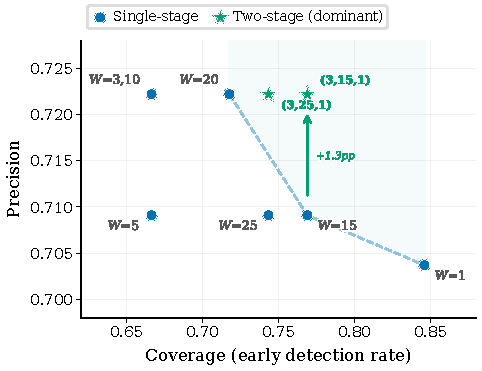
\includegraphics[width=0.85\columnwidth]{figures/pareto_two_stage.pdf}
\caption{Precision-coverage Pareto front comparing single-stage fixed-window detection against two-stage adaptive detection on R1-8B. The best two-stage configuration ($W_{\text{screen}}{=}3$, $W_{\text{confirm}}{=}15$, $k{=}1$) Pareto-dominates single-stage $W{=}15$ by +1.3pp precision at matched coverage. Higher $k$ values shift the tradeoff toward precision at the cost of unacceptable coverage loss.}
\label{fig:pareto_two_stage}
\end{figure}

The marginal improvement suggests that fixed-window smoothing already captures most of the temporal signal available in probe score sequences. The two-stage approach adds configuration complexity (three hyperparameters vs. one) without proportional performance gain.


\section{Temporal Ablation Details}
\label{app:temporal_details}

% Trajectory figure moved to main text §4.5 (Figure: fig_trajectory)

Full per-model temporal ablations are reported in \cref{tab:window_full} (\cref{app:window_ablation}). Key cross-model patterns: (1) R1-8B shows monotonic precision improvement from 69.3\% ($W{=}1$) to 82.2\% ($W{=}25$) with FPR halving (9.65\% to 4.83\%); (2) OT-7B exhibits a split pattern where balanced accuracy peaks at $W{=}3$ while precision and FPR continue improving at larger windows; (3) R1-32B peaks at $W{=}10$ then degrades, likely reflecting overfitting on the small dataset ($n{=}100$); (4) QwQ-32B shows broadly increasing trends with local non-monotonicity. Text probe window ablations (\cref{app:text_window}) show monotonic improvement across all window sizes for both models tested, with larger marginal gains than HS probes (+12.0pp accuracy vs.\ +3.2pp for R1-8B). The asymmetry supports the interpretation that text features benefit proportionally more from temporal context because they encode less information per step.

\section{Negative Results Details}
\label{app:negative_details}

Summary results appear in \cref{tab:negative} (main text); per-method details follow.

\paragraph{BOCPD/CUSUM.} On OT-7B, QwQ-32B, and R1-32B, BOCPD achieves 0\% detection rate across all tested configurations ($\lambda \in \{5, 10, 50, 100, 200\}$). Only R1-8B produces non-zero detection (best: $\lambda{=}10$, 93\% rate, +3.45 steps lead). CUSUM configurations universally underperform simple thresholding on lead time. The probe score sequences for 3/4 models show smooth transitions that never trigger the hazard function (\cref{app:bocpd_config}).

\paragraph{Mahalanobis distance.} Following TrajGuard~\cite{trajguard}, Mahalanobis distance from the pre-CP centroid produces $\Delta d \approx 0$ between pre-CP and post-CP steps. The discriminative signal resides in minor PCA components (explaining $<$5\% of total variance) rather than the principal directions that dominate the distance computation.

\paragraph{RepE.} We compute the mean-difference direction~\cite{zou2023representation} $\mathbf{d} = \bar{\mathbf{h}}_{\text{post}} - \bar{\mathbf{h}}_{\text{pre}}$ from training-set hidden states, then project test-set representations onto $\mathbf{d}$ and threshold the scalar projection. QwQ-32B achieves 0.756 balanced accuracy (approaching supervised 0.778) but with substantially worse precision (0.512 vs.\ LR 0.700) and FPR (0.309 vs.\ 0.120). R1-32B nearly fails (0.559 balanced accuracy). The single direction captures commitment structure in some models but not others, consistent with the multi-dimensional encoding found by \citet{wollschlager2025geometry}.

\paragraph{MLP probes.} Two-layer MLPs ($d \rightarrow 128 \rightarrow 1$, ReLU, no dropout, L2 weight decay $10^{-4}$, early stopping patience 10) underperform logistic regression on 3/4 models. The commitment boundary is linearly separable at correctly selected layers; additional capacity causes overfitting given the small training sets ($n{=}60$--$137$ training examples). All alternative method results in this section are upper-bounded by the hyperparameter search budget reported above.

\paragraph{CCS.} We adapt Contrast-Consistent Search~\cite{burns2023discovering} by constructing contrastive pairs from pre-CP (``safe'') and post-CP (``committed'') hidden states at each reasoning step, then training the CCS probe to satisfy the consistency loss $P(x) + P(\neg x) = 1$. All models required polarity correction (CCS does not determine label direction). CCS achieves 0.692--0.777 balanced accuracy across models but with FPR 0.19--0.41, substantially worse than supervised LR (FPR 0.07--0.28). The consistency objective does not align with temporal commitment structure, and CCS still requires CP labels for pair construction, making it semi-supervised.

\paragraph{Cross-model transfer.} 17 configurations (5 directional pairs $\times$ 3 PCA dimensionalities, plus 2 direct transfers) all fail. Best PCA: R1-8B $\rightarrow$ QwQ-32B at 59.5\% (PCA-2048). Best direct: QwQ-32B $\rightarrow$ R1-32B at 67.3\% but 1\% crossing rate. Implementation details in \cref{app:transfer_details}.

\section{Cross-Model Transfer Implementation Details}
\label{app:transfer_details}

We test whether safety probes transfer across models by projecting hidden states into a shared dimensionality space and applying cross-model classification.

\paragraph{Method.} For each source-target model pair, we apply PCA independently to each model's hidden states, reducing to a shared dimensionality $d \in \{512, 1024, 2048\}$. PCA is fitted on the full dataset (including test traces) for each model separately, a setting favorable to transfer since it maximizes the quality of the projection. A logistic regression classifier (C=1.0, class\_weight=`balanced', max\_iter=2000, random\_state=42) trained on the source model's PCA-projected training data is then applied directly to the target model's PCA-projected test data. No cross-model alignment step (Procrustes rotation, CCA, or learned projection) is applied; PCA serves as a standard linear dimensionality reduction baseline.

\paragraph{Same-dimension pairs.} For R1-32B and QwQ-32B (both 5120-d hidden states), we additionally test direct transfer without PCA: the source classifier is applied directly to the target model's raw hidden states. This tests whether same-architecture, same-dimensionality models share safety-relevant linear structure.

\paragraph{Results.} All 17 transfer configurations (5 directional pairs $\times$ 3 PCA dimensionalities, plus 2 direct transfers for same-dimension pairs) fail to produce practically useful transfer. The best PCA result is R1-8B $\rightarrow$ QwQ-32B at 59.5\% balanced accuracy (PCA-2048). The best direct transfer (QwQ-32B $\rightarrow$ R1-32B) reaches 67.3\% balanced accuracy, which exceeds the within-model baseline of 65.2\%. However, this transfer direction achieves only 1\% crossing rate, meaning the transferred probe almost never triggers detection in practice and is useless for deployment despite above-baseline accuracy. The complete failure under maximally favorable conditions (PCA fitted on full data, no train/test separation for projection) strengthens the conclusion that safety commitment is encoded in model-specific geometric configurations. PCA is a standard linear alignment baseline; its failure indicates that the problem lies in the representations themselves rather than in the choice of alignment method. High balanced accuracy does not guarantee deployment utility: the best direct transfer (67.3\% BA) achieves only 1\% crossing rate, meaning the transferred probe almost never triggers temporal detection despite appearing accurate on per-step classification.


\section{Encoder Robustness Analysis}
\label{app:encoder_robustness}

To test whether the HS advantage over text probes depends on the specific text encoder, we replace all-MiniLM-L6-v2 (384d) with BGE-large-en-v1.5 (1024d), a 2.7$\times$ higher-dimensional encoder with stronger semantic representations. \cref{tab:encoder_robustness} reports precision comparisons at each model's threshold-based layer; \cref{fig:forest_precision} provides a visual summary.

\begin{table}[htbp]
\centering
\small
\caption{HS vs.\ BGE-large (1024d) text probe precision. $\Delta$: HS minus BGE-large. Bootstrap: 10{,}000 resamples, two-sided null-centered. HB: survives Holm-Bonferroni correction (4 tests, $\alpha{=}0.05$).}
\label{tab:encoder_robustness}
\resizebox{\columnwidth}{!}{%
\begin{tabular}{lcccccc}
\toprule
\textbf{Model} & \textbf{HS Prec} & \textbf{BGE Prec} & $\Delta$ & \textbf{95\% CI} & $p$ & \textbf{HB} \\
\midrule
R1-8B & 0.497 & 0.436 & +0.058 & [$-$0.07, +0.20] & 0.185 & No \\
OT-7B & 0.446 & 0.263 & +0.181 & [+0.08, +0.29] & ${<}0.001$ & Yes \\
R1-32B & 0.588 & 0.475 & +0.117 & [$-$0.00, +0.24] & 0.042 & No \\
QwQ-32B & 0.545 & 0.454 & +0.094 & [$-$0.07, +0.28] & 0.132 & No \\
\bottomrule
\end{tabular}}
\end{table}

% Forest plot moved to main text (Figure 4)

The HS precision advantage is directionally consistent across all four models (positive $\Delta$ in every case). OT-7B shows a strong, significant advantage (+18.1pp, $p{<}0.001$, survives Holm-Bonferroni). The remaining three models do not survive Holm-Bonferroni correction; R1-32B's CI includes zero with 10{,}000 resamples, so even the individual precision test is non-significant. This is consistent with the prediction in \cref{sec:limitations} that stronger text encoders would reduce the observed gap. The pattern confirms that the HS modality advantage is genuine but partially attributable to the weakness of the 384d MiniLM baseline.

\paragraph{Balanced accuracy and FPR.} \cref{tab:bge_ba_fpr} reports BGE-large comparisons on balanced accuracy and FPR. HS balanced accuracy advantage is directionally positive across all four models (+8.4 to +10.9pp), with 2/4 (OT-7B, R1-32B) significant under Holm-Bonferroni. FPR advantage is significant only for OT-7B. R1-8B shows an adverse FPR direction: HS FPR is 1.2pp higher (worse) than BGE ($p{=}0.564$), the only model where HS does not improve over the stronger encoder on this metric.

\begin{table}[htbp]
\centering
\small
\caption{HS vs.\ BGE-large (1024d): balanced accuracy and FPR differences. Bootstrap: 10{,}000 resamples, two-sided null-centered. HB: Holm-Bonferroni correction (4 tests per metric, $\alpha{=}0.05$).}
\label{tab:bge_ba_fpr}
\resizebox{\columnwidth}{!}{%
\begin{tabular}{lcccccc}
\toprule
\textbf{Model} & $\Delta$\textbf{BA} & $p$ (BA) & \textbf{HB} & $\Delta$\textbf{FPR} & $p$ (FPR) & \textbf{HB} \\
\midrule
R1-8B & +8.4 & 0.029 & No & $-$1.2$^\dagger$ & 0.564 & No \\
OT-7B & +10.8 & 0.002 & Yes & +10.5 & ${<}0.001$ & Yes \\
QwQ-32B & +9.3 & 0.067 & No & +2.7 & 0.368 & No \\
R1-32B & +10.9 & 0.008 & Yes & +7.8 & 0.165 & No \\
\bottomrule
\end{tabular}}
\begin{flushleft}
\scriptsize $^\dagger$Adverse direction: HS FPR higher (worse) than BGE.
\end{flushleft}
\end{table}


\section{Random Projection Baseline}
\label{app:random_projection}

PCA capacity matching (\cref{app:encoder_robustness}) preserves 79--92\% of variance. A natural question is whether the HS advantage depends on PCA's structure-preserving property. We project hidden states to 384d using Gaussian random projection (3 seeds, averaged) and compare with text embeddings at the same dimensionality (\cref{tab:random_projection}).

\begin{table}[htbp]
\centering
\small
\caption{Random projection (RP, 384d) vs.\ text (384d MiniLM). All $p < 0.001$ (1{,}000 bootstrap resamples). R1-8B uses $W{=}15$ (\cref{tab:hs_vs_text}: $W{=}3$); QwQ-32B evaluated at L60 (\cref{tab:hs_vs_text}: L63). 60/20/20 split.}
\label{tab:random_projection}
\resizebox{\columnwidth}{!}{%
\begin{tabular}{lcccc}
\toprule
\textbf{Model} & \textbf{RP Prec} & \textbf{Text Prec} & $\Delta$\textbf{Prec} & $\Delta$\textbf{BA} \\
\midrule
R1-8B & .621 & .416 & +.205 & +.140 \\
OT-7B & .371 & .244 & +.127 & +.128 \\
QwQ-32B & .563 & .391 & +.172 & +.132 \\
R1-32B & .524 & .441 & +.083 & +.085 \\
\bottomrule
\end{tabular}}
\end{table}

All four models retain significant HS advantage under random projection ($\Delta$Prec +8.3 to +20.5pp), with cross-seed standard deviations below 1.7pp. RP precision is slightly lower than PCA-384d (expected, as PCA preserves maximal variance), but the gap is small. The small gap weakens a pure capacity explanation: even a structure-destroying projection preserves the HS advantage. The safety signal appears broadly distributed across hidden-state dimensions rather than concentrated in top principal components.


\section{LLM-Based Text Encoder Comparison}
\label{app:e5_mistral}

To test whether an LLM-based text encoder closes the HS advantage gap, we encode each reasoning step with E5-Mistral-7B-Instruct~\citep{wang2024e5mistral} (4096d, reduced to 384d via PCA to match the MiniLM dimensionality). \cref{tab:e5_mistral} reports precision comparisons against HS probes at threshold-based layers.

\begin{table}[htbp]
\centering
\small
\caption{HS vs.\ E5-Mistral-7B (PCA 384d) precision. HB: Holm-Bonferroni adjusted (4 tests, $\alpha{=}0.05$). MiniLM precision from \cref{tab:hs_vs_text} for reference. 60/20/20 split.}
\label{tab:e5_mistral}
\resizebox{\columnwidth}{!}{%
\begin{tabular}{llccccccc}
\toprule
\textbf{Model} & \textbf{Layer} & $W$ & \textbf{HS} & \textbf{E5} & \textbf{MiniLM} & $\Delta$(HS$-$E5) & $p$ & \textbf{HB} \\
\midrule
R1-8B & L14 & 3 & .630 & .480 & .416 & +15.0 & 0.001 & \checkmark \\
OT-7B & L16 & 3 & .446 & .321 & .244 & +12.5 & 0.009 & \checkmark \\
R1-32B & L63 & 1 & .588 & .506 & .441 & +8.2 & 0.235 & \\
QwQ-32B & L63 & 5 & .515 & .447 & .391 & +6.8 & 0.368 & \\
\bottomrule
\end{tabular}}
\end{table}

The HS advantage partially survives against the LLM encoder: 2/4 models (both 7--8B) retain significance after Holm-Bonferroni correction. Three text encoders form a monotonic gradient: MiniLM (22M params, 384d): 4/4 HB; E5-Mistral (7B, PCA 384d): 2/4 HB; BGE-large (335M, 1024d): 1/4 HB (\cref{app:encoder_robustness}). E5 precision consistently falls between MiniLM and HS across all models, consistent with encoder quality progressively narrowing the gap. PCA to 384d discards information from the 4096d E5 representation; the comparison controls dimensionality but not representation quality, so the true E5 advantage may be larger than reported here.


\section{Position-Residualized Probing}
\label{app:position_residual}

To quantify non-positional safety signal, we regress out the normalized position $t/T$ from each hidden-state (or text-embedding) vector before training the logistic regression probe. \cref{tab:position_residual} summarizes results across all models at their optimal $W$.

\begin{table}[htbp]
\centering
\small
\resizebox{\columnwidth}{!}{%
\begin{tabular}{lcrrrr}
\toprule
\textbf{Model} & $W$ & \textbf{HS BA} & \textbf{Resid.\ HS BA} & \textbf{Drop} & \textbf{Resid.\ Text BA} \\
\midrule
R1-8B & 15 & 0.834 & 0.669 & 16.5pp & 0.605 \\
R1-8B & 3 & 0.813 & 0.571 & 24.3pp & 0.534 \\
OT-7B & 3 & 0.732 & 0.609 & 12.3pp & 0.540 \\
QwQ-32B & 3 & 0.796 & 0.619 & 17.7pp & 0.582 \\
R1-32B & 1 & 0.756 & 0.552 & 20.4pp & 0.532 \\
\bottomrule
\end{tabular}}
\caption{Position-residualized probe balanced accuracy. All residualized HS probes are above chance ($p{<}0.001$). 3/4 models retain significant non-positional HS advantage over text (gap +3.7 to +6.9pp, HB corrected); R1-32B is the exception (+1.9pp, $p{=}0.914$).}
\label{tab:position_residual}
\end{table}

Position accounts for 12--20pp of balanced accuracy depending on model and window size (R1-32B's 20.4pp drop at $W{=}1$ reflects the absence of temporal context), and all models retain non-positional signal above chance ($p{<}0.001$). Three of four models retain significant non-positional HS advantage over text after residualization (OT-7B +6.9pp, R1-8B +6.4pp at $W{=}15$, QwQ-32B +3.7pp; all HB corrected). R1-32B is the exception: residualized HS-text gap is +1.9pp ($p{=}0.914$), a pattern consistent with position mediation. Larger temporal windows reduce position dependence: R1-8B drops 24.3pp at $W{=}3$ but only 16.5pp at $W{=}15$.

For QwQ-32B specifically, three complementary significance tests confirm the residualized probe performs above chance: Wilcoxon signed-rank $p{=}0.0024$, paired $t$-test $p{=}0.0008$, permutation test $p{<}0.001$ (bootstrap 95\% CI for per-trace BA: $[0.575, 0.744]$). The position baseline achieves higher balanced accuracy (0.832 vs.\ HS 0.796), and HS precision (+4.5pp, $p{=}0.133$) and FPR (+2.5pp, $p{=}0.279$) margins over the position baseline are not statistically significant at $n{=}19$.

\paragraph{Non-linear position terms.}
To test whether non-linear position effects drive the HS advantage, we repeat the residualization with both linear ($t/T$) and quadratic ($[t/T, (t/T)^2]$) regressors (\cref{tab:position_quadratic}). Both 7--8B models retain significant residualized advantages under either specification. R1-32B remains non-significant under both. QwQ-32B's residualized advantage survives linear control (+7.4pp, HB) but is fully absorbed by the quadratic term ($-$1.0pp), indicating a non-linear position component in its HS advantage.

\begin{table}[htbp]
\centering
\small
\resizebox{\columnwidth}{!}{%
\begin{tabular}{lcccc}
\toprule
\textbf{Model} & \textbf{Lin.\ gap} & \textbf{Quad.\ gap} & \textbf{Lin.\ HB} & \textbf{Quad.\ HB} \\
\midrule
R1-8B & +10.4pp & +10.3pp & \checkmark & \checkmark \\
OT-7B & +11.4pp & +9.8pp & \checkmark & \checkmark \\
R1-32B & $-$1.4pp & +0.0pp & $\times$ & $\times$ \\
QwQ-32B & +7.4pp & $-$1.0pp & \checkmark & $\times$ \\
\bottomrule
\end{tabular}}
\caption{Linear vs.\ quadratic position residualization (residualized HS$-$text gap, L60 for QwQ-32B). Both 7--8B models are robust to either specification. QwQ-32B's advantage survives linear but not quadratic control; R1-32B is non-significant under both.}
\label{tab:position_quadratic}
\end{table}

Note: gaps in \cref{tab:position_quadratic} are precision-weighted at per-model optimal layers, whereas \cref{tab:position_residual} reports balanced-accuracy gaps; the difference reflects the metric and layer configuration, not methodological inconsistency.

\paragraph{Effect size.} Standardized effect sizes (Cohen's $d$, residualized per-trace BA vs.\ chance 0.5): R1-8B $d{=}2.37$ ($n{=}43$, very large), QwQ-32B $d{=}0.85$ ($n{=}19$, large). Both exceed the conventional ``large'' threshold of $d{=}0.8$~\citep{cohen1988statistical}, confirming that the residualized HS signal is practically meaningful despite sample limitations at 32B.

\section{Hyperparameter Robustness}
\label{app:hyperparameter_robustness}

The joint search space for layer (${\leq}64$), window $W$ (7 values), consecutive-crossing threshold $K$ (5 values), and decision threshold is large (up to 2{,}240 configurations per model). This raises the concern that reported performance reflects overfitting to small validation sets ($n{=}4$--$9$ per class at 32B). Three analyses address this concern.

\paragraph{Threshold-based metrics converge to a deep-layer band.}
Despite the large search space, three of four threshold-based metrics (precision, inverse FPR, additive composite) independently select L63 (98\% depth) for both 32B models (\cref{tab:layer_selection}). A joint (layer, $W$) grid search over 192 configurations confirms that L63 is near-optimal for QwQ-32B at recommended windows (\cref{tab:joint_layer_w}). For R1-32B, layers L55--L63 at $W{=}1$ form a robust band where all 3/3 metrics pass Holm-Bonferroni (\cref{app:layer_sweep}). The convergence of independent metrics to a narrow band is inconsistent with overfitting, which would produce scattered selections.

\paragraph{BA-optimal layer instability is the finding, not a confound.}
Five-fold cross-validation on 32B validation sets reveals that balanced-accuracy-optimal layers are highly unstable across folds (\cref{tab:fold_ba_layers}). This instability is not a limitation of the study but the central methodological finding: BA-layer selection is sensitive to data composition, and conclusions drawn from any single BA-optimal layer are unreliable. Despite per-fold instability, mean BA across folds peaks near L47--L50 for both models, consistent with the LOO-CV dominant layers (\cref{app:layer_sweep}). The HS advantage holds at both BA-optimal and precision-optimal layers regardless of depth (14/16 per-model tests pass HB; \cref{app:ba_layer_comparison}).

\begin{table}[htbp]
\centering
\small
\caption{BA-optimal layer per fold (5-fold CV, 32B models). Per-fold selections span 24 layers, but mean-BA landscape peaks are stable.}
\label{tab:fold_ba_layers}
\resizebox{\columnwidth}{!}{%
\begin{tabular}{lccccccc}
\toprule
\textbf{Model} & \textbf{F1} & \textbf{F2} & \textbf{F3} & \textbf{F4} & \textbf{F5} & \textbf{Spread} & \textbf{Mean-BA best} \\
\midrule
QwQ-32B & L63 & L51 & L39 & L44 & L44 & 24 layers & L50 \\
R1-32B & L53 & L45 & L40 & L63 & L39 & 24 layers & L47 \\
\bottomrule
\end{tabular}}
\end{table}

\paragraph{Bootstrap CIs quantify statistical uncertainty.}
For the most fragile result (R1-8B FPR), bias-corrected accelerated (BCa) bootstrap~\citep{efron1993bootstrap,carpenter2000bootstrap} yields a 95\% CI of [0.006, 0.159] ($p{=}0.033$), with 12\% leave-one-out instability (\cref{app:multi_seed}). The CI excludes zero and confirms significance despite seed fragility. CP annotation perturbation (\cref{tab:cp_perturbation}) further shows that $\pm 2$-step label noise changes BA by ${<}2.5$pp, so annotation uncertainty does not compound with hyperparameter selection.

\paragraph{Effective degrees of freedom.}
The full exploration space (5 metrics $\times$ 7 windows $\times$ 25--64 layers $=$ up to 2{,}240 configurations) far exceeds the 12 final HB-corrected tests. This does not constitute 2{,}240 independent hypothesis tests because layer and window are selected on the validation set before test-set evaluation, a standard train/validate/test protocol, not post-hoc cherry-picking on test outcomes. The effective degrees of freedom lie between 12 (final tests) and 2{,}240 (full grid), a ``garden of forking paths'' concern~\citep{gelman2013garden}. Three safeguards bound this risk: (1)~nested 5-fold CV on 7--8B models shows 13--25\% shrinkage relative to holdout estimates (\cref{app:nested_cv}), quantifying overfitting; (2)~split-half replication on OT-7B confirms the HS advantage on independent data halves (\cref{app:split_half}); (3)~threshold-based metric convergence to a narrow layer band (L63 for both 32B models) is inconsistent with scattered overfitting selections. We acknowledge that cumulative researcher degrees of freedom are substantial and that the 12-test HB boundary may underestimate Type~I error.

\subsection{Nested Cross-Validation}
\label{app:nested_cv}

The holdout estimates in \cref{tab:hs_vs_text} select layer and window on the validation fold, then evaluate on a fixed test set. To rule out hyperparameter overfitting, we run nested 5-fold cross-validation on both 7--8B models: the outer fold holds out test data; the inner loop selects (layer, $W$) on the remaining four folds. \cref{tab:nested_cv} reports per-fold precision differences.

\begin{table}[htbp]
\centering
\small
\caption{Nested 5-fold CV: per-fold HS$-$text precision difference (pp). Layer and $W$ selected independently per fold. All 10/10 folds favor HS.}
\label{tab:nested_cv}
\setlength{\tabcolsep}{4pt}
\resizebox{\columnwidth}{!}{%
\begin{tabular}{lcccccccc}
\toprule
\textbf{Model} & \textbf{F1} & \textbf{F2} & \textbf{F3} & \textbf{F4} & \textbf{F5} & \textbf{Mean} & \textbf{Holdout} & \textbf{Shrink.} \\
\midrule
R1-8B & +22.1 & +14.4 & +17.5 & +17.0 & +16.0 & $+17.4 \pm 2.6$ & +20.1 & 13\% \\
OT-7B & +13.2 & +21.4 & +18.8 & +12.6 & +15.8 & $+16.4 \pm 3.3$ & +21.9 & 25\% \\
\bottomrule
\end{tabular}}
\begin{flushleft}
\scriptsize R1-8B selected layers: L12, L12, L12, L13, L14; $W_\text{HS}$: 3, 3, 5, 5, 3. OT-7B selected layers: L23, L21, L27, L26, L26 (75--96\% depth); $W_\text{HS}$: 5, 5, 5, 5, 5.
\end{flushleft}
\end{table}

The HS precision advantage is consistent across all 10 folds (5/5 for each model), with mean advantages of +17.4pp (R1-8B) and +16.4pp (OT-7B). Shrinkage relative to holdout estimates is 13\% and 25\% respectively, within expected ranges for validation-selected hyperparameters. R1-8B layer selection is stable (L12--L14, 38--44\% depth), consistent with all five metrics agreeing on L14 in the main analysis. OT-7B nested CV selects L21--L27 (75--96\% depth), deeper than the CR-composite-selected L16 (57\%) used in the main text. The discrepancy between CR-composite-selected (L16) and precision-selected (L21--L27) layers further illustrates the metric-dependence of layer selection documented in \cref{sec:layer-results}.

\paragraph{Formal test.} A one-sided Wilcoxon signed-rank test on the 5-fold $\Delta$precision (HS$-$text) rejects $H_0{:}\;\Delta{=}0$ for both models ($W{=}15$, $p{=}0.031$; the minimum achievable $p$-value at $n{=}5$). Layer selection entropy across folds is $H{=}1.37$ bits for R1-8B (normalized 0.59; dominated by L12 in 3/5 folds) and $H{=}1.92$ bits for OT-7B (normalized 0.83; L21--L27), indicating moderately stable layer selection for R1-8B and higher variability for OT-7B.

\section{Multi-Seed Stability}
\label{app:multi_seed}

\cref{tab:multi_seed} reports LR probe performance across 5 random seeds at each model's threshold-based layer and optimal $W$.

\begin{table}[htbp]
\centering
\small
\caption{LR probe stability across 5 random seeds (threshold-based layers, optimal $W$). 7--8B models are stable; R1-32B shows high variance due to small sample ($n{=}20$).}
\label{tab:multi_seed}
\resizebox{\columnwidth}{!}{%
\begin{tabular}{lccc}
\toprule
\textbf{Model} & \textbf{Precision} & \textbf{Bal.\ Acc} & \textbf{FPR} \\
\midrule
R1-8B & $0.590 \pm 0.072$ & $0.756 \pm 0.028$ & $0.154 \pm 0.026$ \\
OT-7B & $0.421 \pm 0.034$ & $0.633 \pm 0.023$ & $0.157 \pm 0.021$ \\
QwQ-32B & $0.651 \pm 0.099$ & $0.731 \pm 0.028$ & $0.133 \pm 0.032$ \\
R1-32B & $0.594 \pm 0.128$ & $0.692 \pm 0.056$ & $0.207 \pm 0.145$ \\
\bottomrule
\end{tabular}}
\end{table}

R1-32B's high FPR variance (std $= 0.145$) reflects a single outlier seed (FPR $= 0.48$), amplified by the small test set ($n{=}20$). Note that R1-32B's absolute precision std (12.8pp) differs markedly from its paired $\Delta$Prec std (2.0pp): HS and text precision covary across seeds.

\paragraph{5-seed Holm-Bonferroni pass rates.} \cref{tab:seed_hb} reports HB pass rates per model across 5 seeds. Overall, 18/20 (90\%) model-seed combinations pass full HB (3/3 metrics).

\begin{table}[htbp]
\centering
\small
\caption{5-seed HB pass rates (3/3 metrics per seed). R1-8B failures are FPR-specific.}
\label{tab:seed_hb}
\resizebox{\columnwidth}{!}{%
\begin{tabular}{lccc}
\toprule
\textbf{Model} & \textbf{HB Pass} & \textbf{Mean $\Delta$Prec $\pm$ std} & \textbf{Note} \\
\midrule
OT-7B & 5/5 & $+20.9 \pm 1.3$pp & Cleanest evidence \\
R1-32B & 5/5 & $+13.7 \pm 2.0$pp & Position-mediated \\
QwQ-32B & 5/5 & $+19.9 \pm 2.5$pp & Robust \\
R1-8B & 3/5 & $+14.6 \pm 4.5$pp & FPR seed-fragile \\
\bottomrule
\end{tabular}}
\end{table}

\paragraph{R1-8B FPR per-seed breakdown.} \cref{tab:r18b_fpr_seeds} reports per-seed HS vs.\ text FPR comparisons for R1-8B. The HS advantage is directionally consistent (5/5 seeds), with 2/5 reaching $p{<}0.05$ uncorrected; after Bonferroni correction for 5 seeds ($\alpha{=}0.01$), 1/5 remains significant. Text FPR is highly stable (std $= 0.007$) while HS FPR is split-sensitive (std $= 0.040$), which explains why the canonical-split FPR advantage ($-7.4$pp) does not generalize robustly across seeds.

\begin{table}[htbp]
\centering
\small
\caption{R1-8B FPR per-seed comparison (L14, $W{=}15$; main text \cref{tab:hs_vs_text} reports $W{=}3$ after 5-seed validation). Direction is consistent (5/5 HS $\leq$ Text); 2/5 reach $p{<}0.05$ uncorrected, 1/5 after Bonferroni correction (5 seeds, $\alpha{=}0.01$).}
\label{tab:r18b_fpr_seeds}
\resizebox{\columnwidth}{!}{%
\begin{tabular}{ccccc}
\toprule
\textbf{Seed} & \textbf{HS FPR} & \textbf{Text FPR} & $\Delta$\textbf{FPR} & $p$ \\
\midrule
0 & 0.161 & 0.165 & $-$0.004 & 0.440 \\
1 & 0.061 & 0.166 & $-$0.105 & ${<}0.001$ \\
2 & 0.123 & 0.176 & $-$0.053 & 0.093 \\
3 & 0.148 & 0.167 & $-$0.018 & 0.293 \\
4 & 0.100 & 0.176 & $-$0.076 & 0.021 \\
\midrule
mean$\pm$std & $0.119 \pm 0.040$ & $0.170 \pm 0.007$ & $-$0.051 & -- \\
\bottomrule
\end{tabular}}
\end{table}

\paragraph{R1-8B per-metric HB pass rates.} \cref{tab:r18b_metric_hb} reports Holm-Bonferroni pass rates per metric across 5 seeds for R1-8B, the model classified as ``moderate'' evidence due to FPR instability.

\begin{table}[htbp]
\centering
\small
\caption{R1-8B per-metric$\times$seed HB pass rates. Precision is robust (5/5); FPR is fragile (3/5). FPR std across seeds is 0.040 vs.\ text FPR std 0.007, consistent with a proportion near boundary (${\sim}$12\%) amplified at $n{=}43$.}
\label{tab:r18b_metric_hb}
\resizebox{\columnwidth}{!}{%
\begin{tabular}{lccc}
\toprule
\textbf{Seed} & $\Delta$\textbf{Prec HB} & $\Delta$\textbf{BA HB} & $\Delta$\textbf{FPR HB} \\
\midrule
0 & \checkmark & \checkmark & $\times$ \\
1 & \checkmark & \checkmark & \checkmark \\
2 & \checkmark & \checkmark & $\times$ \\
3 & \checkmark & \checkmark & \checkmark \\
4 & \checkmark & \checkmark & \checkmark \\
\midrule
Pass rate & 5/5 & 5/5 & 3/5 \\
\bottomrule
\end{tabular}}
\end{table}

The FPR instability has a clear source: R1-8B text FPR clusters tightly around 17\% (std${=}0.7$pp) while HS FPR ranges from 6.1\% to 16.1\% (std${=}4.0$pp). Seeds where HS FPR happens to be high ($>$14\%) lose significance because the gap against text narrows below the detection threshold at $n{=}43$. This instability is metric-specific and does not affect the precision or balanced accuracy advantage, which passes all 5 seeds.

\paragraph{R1-32B per-seed breakdown.} \cref{tab:r132b_seeds} reports the full per-seed breakdown for R1-32B. Seed 0 is an outlier (FPR $= 0.483$), driven by test-set trace allocation at $n{=}20$. Excluding seed 0, FPR std drops from 0.145 to 0.046.

\begin{table}[htbp]
\centering
\small
\caption{R1-32B per-seed performance (L63, $W{=}1$). Seed 0 is an outlier driven by test-set trace allocation.}
\label{tab:r132b_seeds}
\resizebox{\columnwidth}{!}{%
\begin{tabular}{cccc}
\toprule
\textbf{Seed} & \textbf{Precision} & \textbf{Bal.\ Acc} & \textbf{FPR} \\
\midrule
0 & 0.441 & 0.594 & 0.483 \\
1 & 0.750 & 0.748 & 0.109 \\
2 & 0.685 & 0.670 & 0.111 \\
3 & 0.652 & 0.733 & 0.111 \\
4 & 0.444 & 0.715 & 0.221 \\
\midrule
mean$\pm$std & $0.594 \pm 0.128$ & $0.692 \pm 0.056$ & $0.207 \pm 0.145$ \\
\bottomrule
\end{tabular}}
\end{table}


\subsection{Split-Half Internal Validity (OT-7B)}
\label{app:split_half}

To assess internal validity, we split OT-7B traces into two independent halves and repeat the full layer sweep on each. Both halves reproduce the core pattern: crossing rate selects L0 (shallow) while precision selects mid-to-deep layers (L20 and L26 respectively). The HS precision advantage is consistent across halves ($\Delta$Prec = +0.262 and +0.154), and 4/4 checkpoints (2 halves $\times$ 2 metrics) pass, confirming the metric-induced divergence is not an artifact of a particular data partition (\cref{tab:split_half_ot7b}).

\begin{table}[htbp]
\centering
\small
\caption{Split-half internal validity on OT-7B. Both halves reproduce CR$\to$shallow / threshold$\to$deep divergence with consistent HS advantage direction.}
\label{tab:split_half_ot7b}
\resizebox{\columnwidth}{!}{%
\begin{tabular}{lcccc}
\toprule
\textbf{Half} & \textbf{CR layer} & \textbf{Prec.\ layer} & $\Delta$\textbf{Prec} & $\Delta$\textbf{BA} \\
\midrule
A ($n{=}24$) & L0 & L20 & +0.262 & +0.128 \\
B ($n{=}23$) & L0 & L26 & +0.154 & +0.092 \\
\bottomrule
\end{tabular}}
\end{table}


\section{BA-Layer Modality Comparison}
\label{app:ba_layer_comparison}

To address the concern that threshold-based layer selection may circularly favor HS probes, we repeat the modality comparison at layers selected by pure balanced accuracy, a threshold-free metric (\cref{tab:ba_layer_results}). BA-optimal layers vary widely across models (7--98\% depth), itself demonstrating that layer selection is a consequential methodological choice. The HS advantage is significant at whichever layer BA selects (14/16 per-model HB, two FPR failures from underpowered 32B test sets $n{\leq}20$).

\begin{table}[htbp]
\centering
\small
\caption{HS vs.\ text at BA-selected layers (60/20/20 split, same as main results). 14/16 per-model tests pass Holm-Bonferroni ($\alpha{=}0.05$); two FPR failures from underpowered 32B sets. BA-L: layer selected by pure balanced accuracy. Depth varies from 7\% to 98\%.}
\label{tab:ba_layer_results}
\setlength{\tabcolsep}{3pt}
\resizebox{\columnwidth}{!}{%
\begin{tabular}{lccccc}
\toprule
\textbf{Model} & \textbf{BA-L} & $\Delta$\textbf{Prec} & $\Delta$\textbf{BA} & $\Delta$\textbf{FPR} & $\Delta$\textbf{AUROC} \\
\midrule
R1-8B & L17 & +18.6 ($<$.001) & +8.4 (.006) & $-$7.0 (.043) & +12.1 (.009) \\
OT-7B & L2 & +18.5 ($<$.001) & +8.0 (.006) & $-$13.3 ($<$.001) & +12.8 (.003) \\
QwQ-32B$^\dagger$ & L63 & +18.1 (.001) & +13.5 ($<$.001) & $-$6.4 (.088) & +15.1 (.001) \\
R1-32B$^\dagger$ & L46 & +12.8 (.014) & +17.6 ($<$.001) & $-$12.2 (.083) & +15.1 (.009) \\
\bottomrule
\end{tabular}}
\begin{flushleft}
\scriptsize Values: difference in pp ($p$-value, bootstrap, 10{,}000 resamples). $\dagger$\,Sample-limited ($n \leq 20$).
\end{flushleft}
\end{table}

Of 16 per-model tests (4 models $\times$ 4 metrics), 14 pass Holm-Bonferroni correction. The precision gains (+12.8 to +18.6pp) are comparable to those at threshold-based layers (+15.4 to +21.9pp; \cref{tab:hs_vs_text}), so the HS advantage is robust to the choice of layer selection criterion. The two failures are both FPR at 32B: R1-32B ($p{=}0.083$) and QwQ-32B ($p{=}0.088$), consistent with the underpowered test sets ($n{\leq}20$) noted throughout. BA-optimal depths span 7\% (OT-7B L2) to 98\% (QwQ-32B L63), in contrast to threshold-based layers that consistently select deep layers (94--98\%). That BA selection produces such depth variation while preserving significant HS advantage reinforces the core methodological finding: the advantage is genuine rather than an artifact of any particular layer selection criterion.


\subsection{AUROC Layer Selection}
\label{app:auroc_layer}

AUROC is threshold-free and thus orthogonal to the threshold-based metrics used in our main analysis. We include it as a reference point for layer selection (\cref{tab:auroc_layer}).

\begin{table}[htbp]
\centering
\small
\caption{AUROC-optimal vs.\ threshold-based layer selection. AUROC selects mid-depth layers for 32B models (${\sim}$50\%), diverging from threshold-based deep layers ($>$90\%). PCA-256 applied to 32B models for tractability.}
\label{tab:auroc_layer}
\setlength{\tabcolsep}{3pt}
\resizebox{\columnwidth}{!}{%
\begin{tabular}{lcccccc}
\toprule
\textbf{Model} & \textbf{AUROC-L} & \textbf{Depth} & \textbf{AUROC} & \textbf{Thresh-L} & \textbf{Depth} & \textbf{AUROC@Thresh-L} \\
\midrule
R1-8B & L13 & 41\% & 0.806 & L14 & 44\% & 0.803 \\
OT-7B & L1 & 4\% & 0.777 & L16 & 57\% & 0.746 \\
QwQ-32B$^\dagger$ & L32 & 50\% & 0.839 & L60 & 94\% & 0.756 \\
R1-32B$^\dagger$ & L31 & 48\% & 0.897 & L63 & 98\% & 0.767 \\
\bottomrule
\end{tabular}}
\begin{flushleft}
\scriptsize $\dagger$\,PCA-256 applied. AUROC-L: layer maximizing validation AUROC. Thresh-L: layer from threshold-based selection (\cref{tab:layer_selection}).
\end{flushleft}
\end{table}

AUROC does not converge to the same deep layers as threshold-based metrics. For 32B models, AUROC prefers mid-depth layers (${\sim}$50\% depth) vs.\ threshold-based deep layers ($>$90\%). R1-8B is a near-match (L13 vs.\ L14). We exclude AUROC from the main analysis because it is threshold-free and cannot diagnose the threshold-crossing artifacts central to our layer selection bias finding, but it provides an independent reference confirming that optimal layer depth is metric-dependent.\looseness=-1

\subsection{Effective Independent Tests}
\label{app:effective_tests}

The raw exploration space (${\sim}$5 metrics $\times$ 7 windows $\times$ 28--64 layers) nominally spans 980--2{,}240 configurations per model, raising a multiple-comparisons concern. The effective number of independent tests is substantially smaller for three reasons:

\paragraph{Metric redundancy.} Precision, inverse FPR, and the additive composite share a single confusion matrix: they are deterministic functions of the same TP/FP/FN/TN counts. Empirically, their layer rankings have Kendall $\tau \geq 0.85$ across all four models (\cref{tab:layer_selection}). BA is computed from the same confusion matrix but weights errors differently; it independently confirms deep-layer selection. Crossing rate is the only structurally distinct metric (computed from threshold-crossing sequences, not the confusion matrix). Thus five nominal metrics reduce to ${\sim}$2 independent metric families (threshold-based and crossing-rate).

\paragraph{Layer autocorrelation.} Adjacent transformer layers produce highly correlated probe scores: for R1-8B, the median Pearson $r$ between layers $\ell$ and $\ell{\pm}1$ exceeds 0.95. Using a lag-1 autocorrelation estimate~\citep{efron1993bootstrap}, the effective number of independent layers is ${\sim}$8--12 per model (vs.\ 28--64 nominal).

\paragraph{Two-stage protection.} The upstream exploration (layer $\times$ window $\times$ metric) is conducted entirely within the training/validation split via nested CV at 7--8B (\cref{app:nested_cv}) and split-half replication (\cref{app:split_half}). The held-out test set sees only the 12 final modality comparisons (3 metrics $\times$ 4 models), to which Holm-Bonferroni correction is applied. The upstream search inflates Type I risk only if it overfits the validation set; nested CV guards against this at 7--8B, while 32B results are marked exploratory ($\dagger$) precisely because this guard is unavailable.

\paragraph{Conditional inference.} The two-stage design means that test-set $p$-values are conditional on the layer and window selected during upstream search. This selective inference is valid when the selection and evaluation splits are independent (ensured by our 60/20/20 partition), but the resulting $p$-values measure significance given the chosen selection path rather than significance averaged over all possible paths. Nested CV at 7--8B (\cref{app:nested_cv}) addresses this by averaging over fold-specific selection paths; the 32B exploratory status ($\dagger$) reflects the absence of this protection.

\paragraph{Effect sizes.} Cohen's $d$ (one-sample, $d = (\overline{\text{BA}} - 0.5) / s$) quantifies effect magnitude independently of sample size: R1-8B $d{=}2.37$ (very large, $n{=}43$), OT-7B $d{=}1.12$ (large, $n{=}47$), QwQ-32B$^\dagger$ $d{=}0.85$ (large, $n{=}19$), R1-32B$^\dagger$ $d{=}0.58$ (medium, $n{=}20$). The 7--8B models exceed the ``very large'' threshold ($d{>}1.2$); both 32B models exceed the ``medium'' threshold ($d{>}0.5$). R1-32B's medium effect size is consistent with its exploratory status and the position-mediation pattern noted in \cref{sec:32b-analysis}. These effect sizes argue against a pure multiple-comparisons explanation: fishing artifacts produce small, unstable effects, whereas the observed $d$ values are large and graded across the evidence tiers.\looseness=-1

\section{Post-Hoc Power Analysis}
\label{app:power_analysis}

We compute post-hoc minimum detectable effects (MDEs) at 80\% power for each model's test set to contextualize non-significant results, particularly at 32B scale where sample sizes are small (\cref{tab:power_analysis}).

\begin{table}[htbp]
\centering
\small
\caption{Post-hoc power analysis. MDE: minimum detectable effect (balanced accuracy, pp) at 80\% power given each model's test-set size and observed variance. Effects smaller than the MDE cannot be reliably detected.}
\label{tab:power_analysis}
\resizebox{\columnwidth}{!}{%
\begin{tabular}{lccc}
\toprule
\textbf{Model} & $n_{\text{test}}$ & \textbf{Obs.\ std (BA)} & \textbf{MDE (80\%)} \\
\midrule
R1-8B & 43 & 0.028 & 4.2pp \\
OT-7B & 47 & 0.023 & 3.3pp \\
QwQ-32B$^\dagger$ & 19 & 0.028 & 8.6pp \\
R1-32B$^\dagger$ & 20 & 0.056 & 9.5pp \\
\bottomrule
\end{tabular}}
\begin{flushleft}
\scriptsize $\dagger$\,Sample-limited. MDE computed from 5-seed observed standard deviation via two-sided paired $t$-test formula.
\end{flushleft}
\end{table}

At 32B scale, the MDE is 8.6--9.5pp, meaning effects below this magnitude cannot be reliably distinguished from noise. R1-32B's residualized HS-text gap (+1.9pp) falls well below the MDE (9.5pp), so the non-significant result (\cref{app:position_residual}) is consistent with either a true null or an underpowered test. The 7--8B MDEs (3.3--4.2pp) are substantially lower, explaining why smaller effects reach significance at these scales.

\subsection{Multi-Metric Layer Ensemble}
\label{app:ensemble}

Results appear in \cref{tab:ensemble} (main text); methodological details follow.

For each model, we train logistic regression probes at the best layer selected by each of three threshold-based metrics (precision, BA, inverse FPR) and average their predicted probabilities to produce an ensemble score. This eliminates the need to pre-select a single metric for layer selection.

This ensemble is a preliminary exploration of metric-agnostic layer selection, not a validated mitigation strategy; rigorous cross-validated evaluation across diverse datasets is future work. The ensemble provides a metric-agnostic selection strategy among principled (threshold-based) metrics. It never significantly underperforms the best individual metric (all $p > 0.27$), and all four models show significant HS advantage over text ($p \leq 0.002$). The ensemble advantage over text ranges from +10.5pp (R1-32B) to +27.0pp (OT-7B). This proof of concept validates that practitioners need not commit to a single metric for layer selection; averaging across metric-selected layers achieves comparable performance. Future work should test whether including biased metrics (e.g., crossing-rate composite) in the ensemble degrades performance, and whether learned metric weighting could improve upon uniform averaging.

\subsection{Practical Mitigation Levels}
\label{app:practical_mitigation}

We propose a three-level defense against metric-induced layer selection bias.

\emph{Level~1 (minimal)}: report layer selections under both threshold-based and frequency-based metric families; divergence exceeding 20\% of model depth (e.g., L2 vs.\ L63 in a 64-layer model) indicates metric-induced bias and warrants treating conclusions as provisional.

\emph{Level~2 (recommended)}: a multi-metric audit (\cref{app:deployment_operating_points}) computes all five metrics and flags when ${\geq}3$ select layers differing by ${>}20\%$ of depth, an operational test requiring no additional data.

\emph{Level~3 (robust)}: a three-layer ensemble averaging probe predictions from the precision-best, BA-best, and inverse-FPR-best layers eliminates metric pre-selection entirely ($p \leq 0.002$; \cref{tab:ensemble}), but requires cross-validated confirmation before deployment.

\section{32B Model-Specific Analysis (Full)}
\label{app:32b_full}

Results are exploratory ($n{=}19$--$20$; MDE at 80\% power: 8.6--9.5pp; \cref{app:power_analysis}). Both 32B models lack nested CV; LOO-CV and multi-seed analyses (\cref{app:layer_sweep,app:multi_seed}) provide partial robustness checks. R1-32B$^\dagger$ suggests commitment 11--13 steps early (coverage 25\%, $W{=}1$ only; +14.2pp over position baseline, HB; precision +15.4pp); the residualized gap (+1.9pp) is below MDE. QwQ-32B$^\dagger$ achieves significance at all window sizes (74\% coverage, HB) but with negative lead time ($-$1.2 to +1.9 steps); the position baseline achieves higher BA (0.832 vs.\ 0.796, +3.6pp, $p{=}0.133$, NS; \cref{app:position_residual}). Despite sharing the Qwen-32B architecture, the two models present opposite profiles; replication with $n{\geq}50$ traces is needed.

\section*{Use of AI Assistants}
\addcontentsline{toc}{section}{Use of AI Assistants}
\label{app:ai-assistants}

We used Claude (Anthropic) as an AI coding and writing assistant throughout this work. Specifically:
\begin{itemize}
    \item \textbf{Code:} drafting experiment scripts, data-processing pipelines, and analysis utilities; debugging and refactoring.
    \item \textbf{Writing:} drafting and revising paper sections, polishing prose, and reformatting LaTeX.
    \item \textbf{Literature:} summarizing related papers to inform the related-work section.
\end{itemize}

